Two primary motivations drive the exergy analysis described below.  The primary motivation behind this research is to demonstrate the differences in revenue generated between thermally and electrically coupling water purification systems to nuclear power plants in a \ac{nrhes} configuration.   An additional motivation is \ac{aps}, which owns about 29\% of \ac{pvgs} as well as operates the power plant, is evaluating electrically coupling a reverse osmosis system.  The \ac{ro} system will allow Palo Verde to vary the amount of electricity sent to the electric grid while generating water to meet the power plant's own water requirements in addition to increasing the water resources available for communities in the surrounding region.

Due to a high penetration of solar energy, Arizona is an ideal setting to examine the possibilities of a \ac{nrhes}. Arizona has been a leader in implementing solar electricity. In 2013, Arizona produced 23.4\% of all US solar generation and 1.9\% of the electricity within the state.  By 2016, solar in Arizona nearly doubled production to 3.4\% of the total electricity for the state. The state also has a renewable portfolio standard requiring 15\% renewable energy by 2025 from regulated utilities\cite{DSIRE2017}, including \ac{aps}. With an increasing penetration of solar in the state, other sources of generation will have to operate more flexibly to account for the variable generation. Furthermore, when California produces more electricity than that state demands, much of the overproduction is sent to Arizona either for free or California pays Arizona to take the overproduction \cite{Penn2017}. The overproduction of electricity by variable sources is only likely to increase with the California Legislature's mandate that half of the state's electricity come from renewable sources by 2030 \cite{Penn2017} and Arizona's ballot measure to raise the states renewable energy standard to demand 50\% of utility electricity come from renewables by 2030 \cite{Ballotpedia2018}.

\ac{pvgs} generates more electricity than any other power plant in the entire United States. In January 2018, Palo Verde produced 36.37\% of Arizona's power \cite{eia2018}.  As such a large contributor to the Arizona grid, Palo Verde fluctuating could counterbalance the large shifts in solar power generated during the day and unavailable during the evening and night hours. The motivation for \ac{pvgs} is to ensure the plant is not loosing money by selling electricity for less then it costs the plant to generate during certain times in the day. Palo Verde has a zero discharge water cycle.  Zero discharge means that, unlike most nuclear power plants that release heated water into a body of water, all of the water at Palo Verde either stays at the power plant forever or is evaporated from the evaporation ponds or the cooling towers.  The power plant uses waste water from Phoenix's 91st avenue treatment facility and Tolleson's water treatment facility. At the time of Palo Verde's initial operation in 1986, the treated waste water was not worth very much, but with the increasing unavailability of water and population growth in Arizona, water has become more valuable \cite{Brown2018}.  Arizona has significant amounts of brackish groundwater that could be pumped up from underground aquifers and used in place of the treated waste water currently in use at Palo Verde. The general composition of Arizona's brackish groundwater can be seen in Table \ref{ArizonaWater}.

\begin{table}[h!]
\centering
\caption{The Components of Brackish Groundwater in Central Arizona Centerra Well from \cite{USBureauofReclamation2006}}
\label{ArizonaWater}
\begin{tabular}{|l|l|}
\hline
\textbf{Material}                                                & \textbf{Mole Percent} \\ \hline
Calcium  & 7.32E-3     \\ \hline
Magnesium & 5.11E-3      \\ \hline
Sodium & 3.24E-2\\ \hline
Sulfate & 9.47E-3 \\ \hline
Barium & 5.25E-6 \\ \hline
Nitrate & 5.20E-4 \\ \hline
Flouride & 6.64E-5 \\ \hline
Arsenic & 7.21E-8 \\ \hline
Water                                                      & 99.9         \\ \hline
\end{tabular}
\end{table}

Palo Verde is pursuing a water purification facility in order to ensure a reliable and cost effective source of water for the power plant while also providing the surrounding communities with sufficient water to sustain growth. While Palo Verde is planning an electrically coupled reverse osmosis system, it is worth knowing what kind of water output would be expected from a thermally coupled system for future plants interested in pursuing desalination and water purification. Furthermore, it provides an initial model and point of reference for determining the benefits of thermally coupling as compared to electrically coupling water purification systems. Having seven separate owners has led Palo Verde in the direction of an electrically coupled \ac{ro} system, as discussed below. Since APS owns about 29.1\% of the facility, it owns about 29.1\% of the load generated from the facility. \ac{aps} has a total entitlement of about 1146 MW from Palo Verde \cite{PinnacleWestCapitalCorporation2016}. APS can allocate the electrical load it owns as desired to the \ac{ro} system in order to flexibly operate the electric load it sells to the grid as well as to ensure lower costs of water for the power plant. Even if using waste heat, thermal coupling to a reactor would impact the power cycle of the plant, as discussed in the results.  Thermally coupling any industrial process to a nuclear power plant, will require changes in the power cycle.  To have sufficient heat for even a low temperature process, some heat will have to be taken away from power generation. To avoid the complications of determining the technical as well as policy implications of thermally coupling with six owners, APS is opting for simplicity by pursuing an exclusively electrically coupled system \cite{Brown2018}.

This analysis will focus on three major benefits of coupling Palo Verde to a water purification system.  One of the primary benefits is load following by sending excess power at times when electricity is cheap to produce clean water. Second, the system can optimally use the heat produced by the reactor to produce the greatest revenue. Finally, by \ac{aps} owning the means of water production, the cost of water would be easier to predict and reliable.

The literature review presented at the beginning of this thesis revealed a notable gap in the current research modeling the benefits gained from thermally coupling compared to electrically coupling industrial processes. Thermal coupling refers to using the heat directly from the \ac{npp} in industrial processes as opposed to generating electricity, which is then used by industrial processes. Fully determining the benefits of thermal coupling requires complicated analyses that are beyond the scope of this research. The full answer requires research focused on particular projects including economic, technical, as well as political and cultural factors. The goal for this research is to address some of the possible thermodynamic and economic benefits of thermally coupling nuclear power to a water purification system at a high level focusing strictly on revenue.

The major drawbacks of thermally coupling any industrial process to a \ac{npp} are the increase in system complexity and the lack of experience in the domain. While there are cases of thermal coupling of nuclear power plants internationally, in Norway, Switzerland, Germany, and Canada \cite{Verfondern},  nuclear thermal couplings are as of yet undeveloped in the United States.  The low state of development as well as the lack of experimental data in the United States has created a lack of data and maturity of experience as a base for building such systems.  The uncertain regulatory environment regarding thermally coupled \ac{nrhess} and whether they fall under the \ac{nrc}'s umbrella also discourages development.

The success of thermally coupled systems requires that their efficiency benefits be greater than the costs associated with developing and operating thermal coupling nuclear generation and co-locating industrial processes.  An exergy analysis of both the electrically coupled and thermally coupled industrial processes provides a quantitative measure of the thermodynamic benefits of thermally coupling. The fuzzy AHP analysis concluded that, given the characteristics of safety, flexibility, and profitability, the optimal industrial process is desalination. Based on this analysis, the exergy evaluation will focus on two desalination systems.  The thermally coupled system in this analysis is \ac{msf} distillation, which will be compared to an electrically coupled \ac{ro} system. The research concludes that, while thermally coupling is thermodynamically better, electrically coupling has significant benefits in terms of flexibility, modularity, and is fairly close in thermodynamic exergy values when not much water is required.

\section{Exergy Analysis Background}
The concept of exergy is helpful for analyzing the energy allocation in a system. Exergy, also known as availability, describes the energy available in the system for doing work. Exergy has the same units as energy, most commonly Joules. Exergy destruction occurs when energy is either used for doing work or through inefficiencies in the system.  By evaluating where exergy is destroyed and the economic value the product of the exergy destruction, in this case either electricity or clean water, a hybrid energy system can be optimized for revenue. An exergy analysis can identify available exergy that used to be released into the environment that could instead be used to do the work required in a water purification system.

Exergy describes the useful energy in a system for generating work. The first and second laws of thermodynamics clarify that not all the energy generated in a system can be converted into usable work.  The first law describes how energy cannot be created or destroyed, it can only be converted into a different form.  For example, chemical combustion in a fire produces heat and light. The second law states that entropy can only increase in a system. Entropy is often thought of as the amount of randomness in a system.  Having disorder or randomness in a system requires energy that cannot be used to generate work. The entropy of a system is the energy used in the system working towards reaching a state of equilibrium.  For example, assuming a system is a room at 70\degree F with a glass of ice in it, some energy will go towards bringing the glass to the same temperature as the surrounding environment. This energy is called the entropy in the system. Some energy always goes towards the entropy in the system, making it unusable, for example, to produce electricity.


Exergy can be a more descriptive metric than energy loss as it describes how close a system is to an ideal design with the least physical possible energy losses across the system. In order to determine the maximum possible energy efficiency of a power cycle requires finding the Carnot efficiency $\eta_{Carnot}=1-\frac{T_0}{T}$. The Carnot efficiency describes the maximum possible output of a system. It is physically impossible for the Carnot efficiency to equal 100\%.  Anything above the Carnot efficiency of a cycle, which is the ideal theoretic output of a system, which would be a perpetual motion machine.  Systems will always lose energy through entropy. The exergy efficiency describes how much of the energy available to do work is transferred by the system into useful work or how effective the cycle is designed to extract all of the available energy. The exergy analysis in this research evaluates the exergy lost in the power cycle as well as the exergy lost when using the pumps. The exergy analysis can then be combined with an economic analysis determining when the greatest value is generated for each unit of exergy destroyed. For this project, the exergy analysis will include the components modeled in Palo Verde's Rankine Power Cycle as well as the water purification systems.

In an ideal reversible process, no exergy would be lost or entropy generated. Reversible processes are ideal processes that can restore the system to its initial state when the process is reversed without any external energy added to the system. No processes are fully reversible in reality. Irreversible processes increase the entropy in the system, thereby removing some of the exergy in the system. Finding where exergy is destroyed in a system can help indicate where losses are occurring. By applying an economic exergy analysis, the system can be optimized so that the exergy losses are incurred in the most valuable way possible.

The basic mass exergy equation of a system is \cite{moran2010fundamentals}:

\begin{equation}
\triangle X=(U-U_0)+p_0(V-V_0)-T_0(S-S_0)+KE+PE
\label{Xergy}
\end{equation}
\\
Where $\triangle X$ is the change in the exergy of the system from the exergy reference environment in kJ.  Exergy is rarely based off of a state of 0 K, but is instead a reference value as compared to some environment from which it differs. $U$ is the internal energy of the system and $U_0$ is the reference internal energy of the system both in kJ. $p_0$ is the reference pressure of the system in kPa, $V$ is the volume of the system and $V_0$ is the volume of the reference environment both in $m^3$. $T_0$ is the reference environment temperature given in K, $S$ is the entropy of the system and $S_0$ is the entropy of the reference environment in $\frac{kJ}{K}$. $KE$ is the kinetic energy of the system in kJ equal to $\frac{1}{2}m*v^2$ where $m$ is mass and $v$ is the velocity of the system. $PE$ is the potential energy in kJ equal to $mgh$ where $g$ is the gravitational constant and $h$ is the height of the system. The specific exergy of the system, or the exergy of the system not including the mass, is displayed as $x$.  To find the specific exergy of the system, each of the elements in the equation are divided by the mass, which is in kg in this case. Specific thermodynamic properties differ from mass thermodynamic properties in that the specific values are characteristics of the materials regardless of mass. The resulting equation for internal exergy is:

\begin{equation}
\label{specificX}
\triangle x=(u-u_0)+p_0(v-v_0)-T_0(s-s_0)+\frac{1}{2}v^2+gh
\end{equation}
\\

The elements now represent the specific values of the system with the same units as above but per unit mass as opposed to the mass dependent variables shown in equation \ref{Xergy}.  For this research, the mass based values will be neglected, focusing instead specifically on the internal exergy values. The internal exergy differences thoroughly describe the system.  The mass transfer within either the power cycle or the water purification systems does not provide any extra insight into the relative magnitude of exergy loss in the various components. The kinetic energy term, $\frac{1}{2}v^2$, is negligible due to the relatively low velocity of the system making the $KE$ small compared to the other terms in the equation thus ignorable.  The potential energy element, $gh$, is negligible throughout the system. The enthalpy, $h$, of a system, or the total heat content of the system, is equivalent to the specific internal energy plus the pressure multiplied by the change in specific volume.  Put mathematically:

\begin{equation}
\triangle h=(u-u_0)+p_0(v-v_0)
\end{equation} Including enthalpy in place of the first two elements in equation \ref{specificX} as well as removing the last two elements leaves the specific exergy equation, which is applied in this research, as simply:

\begin{equation}
\triangle x=(h-h_0)-T_0(s-s_0)
\end{equation}

\subsection{Relevant Exergy Analysis Research}
Boldon et al. have already performed an initial exergy analysis on a \ac{nrhes}, assuming a SMR \cite{Boldon}. Boldon et al. discuss the value of combining exergy and economics to analyze costs associated with exergetic losses. The assumptions in the Boldon et al. paper include a steady state system with a constant grid output of 245 MWe.  The nuclear plant is both thermally and electrically coupled to a High Temperature Steam Electrolysis industrial process. After performing the thermodynamic exergy analysis, Boldon et al. incorporate costs of resources and operations, enabling them to assign an exergetic unit cost to each of the components in the system.

The exergy analysis in this paper differs from Bolden et al. by analyzing an existing large nuclear power plant, focusing on water purification methods, including a quasi dynamic analysis, and, most importantly, focusing on revenues as opposed to costs.  An exergoeconomic cost analysis can provide relevant information to determining the price of the products generated, but it does not include the known values for the price of the products. The revenue derived from the products of the system will dictate the \$/exergy as opposed to the costs of the system.

%In order to include a quasi dynamic approach, both the MSF and RO systems are evaluated on the optimal \$/exergy costs and will also take into consideration the load following capabilities valuable to \ac{aps} through determining at what price for water and electricity it would be valuable to switch to generating water.

An exergetic analysis of the Kalundborg industrial ecosystem, a non nuclear hybrid energy system, evaluates the streams going into and out of the Asnaes power plant \cite{Valero2012}.  Valero et al. contrast the exergy of the coupled system with an uncoupled system. As can be seen in figure \ref{Kalendburg}, the Kalundborg industrial ecosystem is comprised of the Statoil refinery, the Asnaes coal power plant, the Novo Group pharmaceutical company, district heating for local residents, the Gyproc plasterboard manufacturer, as well as a fish farm and the Aalborg Portland cement company. The major exergetic gains for the system come from sharing process heat from the natural gas from the refinery, district heating, heating the fish farm, and using clinker (a coal plant byproduct) to produce cement \cite{Valero2012}. The overall reduction in irreversibilities annually from coupling the systems at Kalundborg amounts to approximately 1476 GWh/year, the equivalent of the annual production of a 170.235 MW power plant. By comparing the exergy of a coupled system with the separate industrial processes, the Kalundborg example provides insight into the thermodynamic and economic benefits of co-locating processes. Figure \ref{Kalendburg} displays the two different approaches taken; first evaluating the exergy of the combined systems, then evaluating the separate processes.

\begin{figure*}
\centering
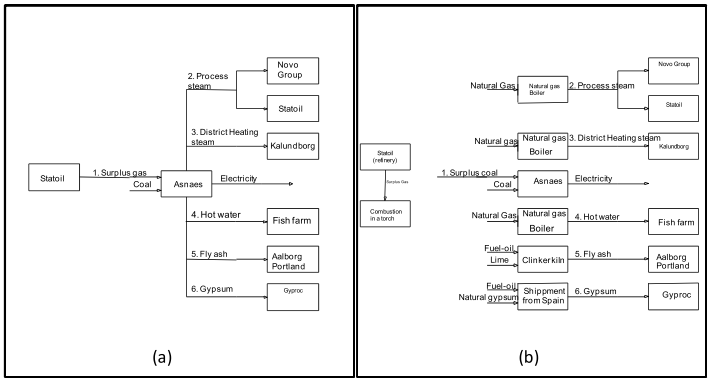
\includegraphics[width=\textwidth]{kalundborg_cases.PNG}
\caption{\small \sl This figure displays the two cases evaluated in Valero et al.: (a) shows the industrial ecosystem in the current coupled form and (b) shows the second case where there is no coupling.}
\label{Kalendburg}
\end{figure*}


\subsection{Multi-Stage Flash Distillation}
As the \ac{nrhess} evaluated for this thesis includes a \ac{msf} distillation system, a brief review of a MSF distillation exergy analysis is included. Kahraman et al. performed an exergy analysis on a large MSF plant \cite{Kahraman2005}.  \ac{msf} distillation requires heat ranging from 80 to 120 degrees Celsius, making it possible to use high temperature waste heat from a nuclear power plant to desalinate or purify the water. In general, the waste heat coming from a nuclear power plant is significantly below 100\degree C. Extra heat would thus need to be sent to the environment, in this case the MSF process, in order for the waste heat to fully power the MSF process. The same processes, RO and MSF, can be used for both water purification and desalination, so the terms can be used fairly interchangeably. In the case of Palo Verde, the system is a water purification system for brackish groundwater. In the exergy analysis, Kahraman et al. takes the temperature of the salinated water to be the assumed reference environmental conditions for the system, making the initial exergy zero. Similarly, in the exergy performed in this thesis, the assumed reference environmental conditions are taken as the temperature of the water intake. Kahraman et al.'s exergy analysis includes finding the exergy of the heat exchanger and four pumps in the system, as well as calculating the difference in exergies between the incoming water and the exiting pure water. The analysis is used to find the overall exergy efficiency and determine where to reduce exergy destruction in the system.

Figure \ref{MSF_x} displays where exergy is destroyed in the MSF system. Clearly the majority (77.7\%) of the exergy is destroyed in the MSF distillation system itself. Other sources of irreversibilities include the inefficiencies and losses due to the pumps and heat exchangers as well as the final release of the waste brine water to the environment. The exergy destroyed in the MSF system went to a process that produced a valuable product.  The other sources of exergy destruction are physically necessary losses with no economic benefits. In the economic exergy study performed in this thesis, the exergy destruction will be evaluated based on its economic value.  Both generating pure water in the MSF system as well as producing and using electricity for the reverse osmosis system result in exergy destruction.

\begin{figure*}[h!]
\centering
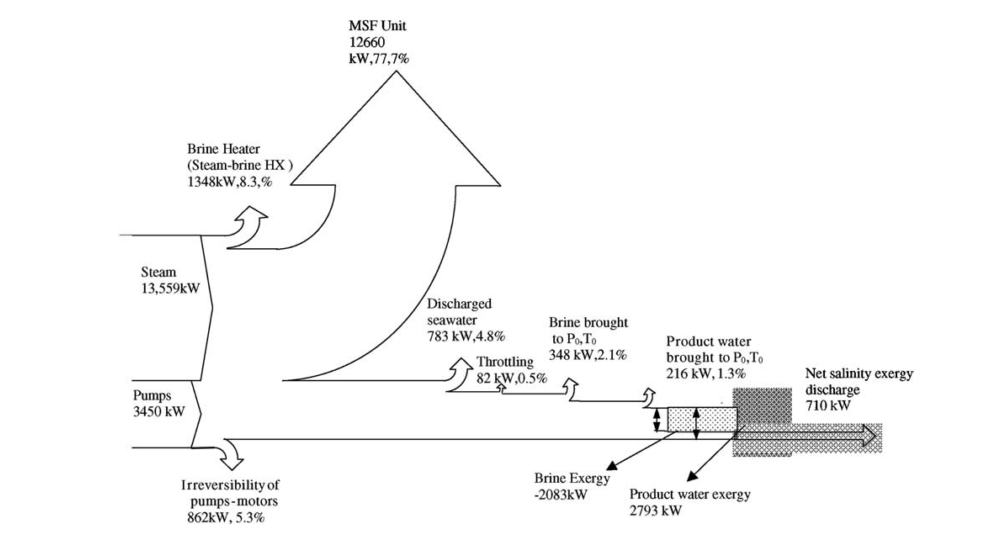
\includegraphics[width=\textwidth]{MSF_exergy.PNG}
\caption{\small \sl The Multi-Stage Flash exergy analysis diagram showing where exergy is lost in the system.  This exergy diagram was published in \cite{Kahraman2005}}.
\centering
\label{MSF_x}
\end{figure*}

MSF is a common thermal desalination system, making up about 21\% of the total worldwide installed capacity as can be seen in figure \ref{DesalData}. In an MSF system, salt water or brackish water is flash evaporated, then condensed repeatedly in order to remove unwanted particulates. As can be seen in figure \ref{salinity}, brackish water has more salinity or impurities than fresh water, but not as much as sea water. MSF can produce clean water in large quantities, with plants in Saudi Arabia and the United Arab Emirates having capacities of 600,000-880,000 $m^3/day$ \cite{El-Dessouky2016}. In general, an MSF system works by passing sea water or brackish water through a series of chambers, each with successively lower temperature and pressure.  The water is quickly flashed, or vaporized.  The water, without the brine, is then condensed, forming freshwater.  The stages can range widely, depending on the concentration of the feedwater brine and the desired state of purity for the freshwater. Standard sizes for fairly large MSF arrays range from 21 to 50 stages. Generally, MSF distillation is a mature technology used for high capacity desalination systems. The major benefit of \ac{msf} as compared to other water purification methods is the high level of purity of the water.
\begin{figure*}[h!]
\centering
\label{DesalData}
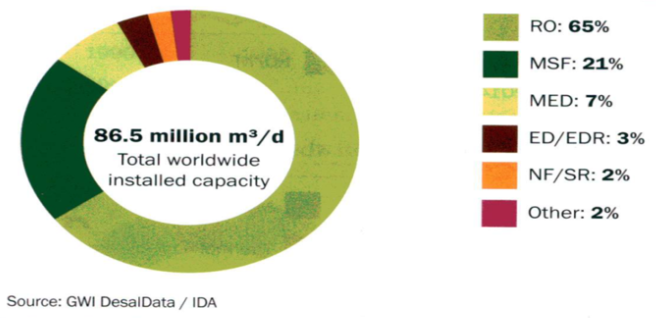
\includegraphics[width=\textwidth]{DesalData.PNG}
\caption{\small \sl This pie chart from \cite{Khamis} shows the overall total installed capacities of each of the technologies used for desalination. The six technologies shown represent Reverse Osmosis (RO), Multistage Flash (MSF), Multiple-effect distillation (MED), Electrodialysis Reversal (ED/EDR), and Nanofiltration (NF)}
\centering
\label{DesalData}
\end{figure*}



\begin{figure*}[h!]
\centering
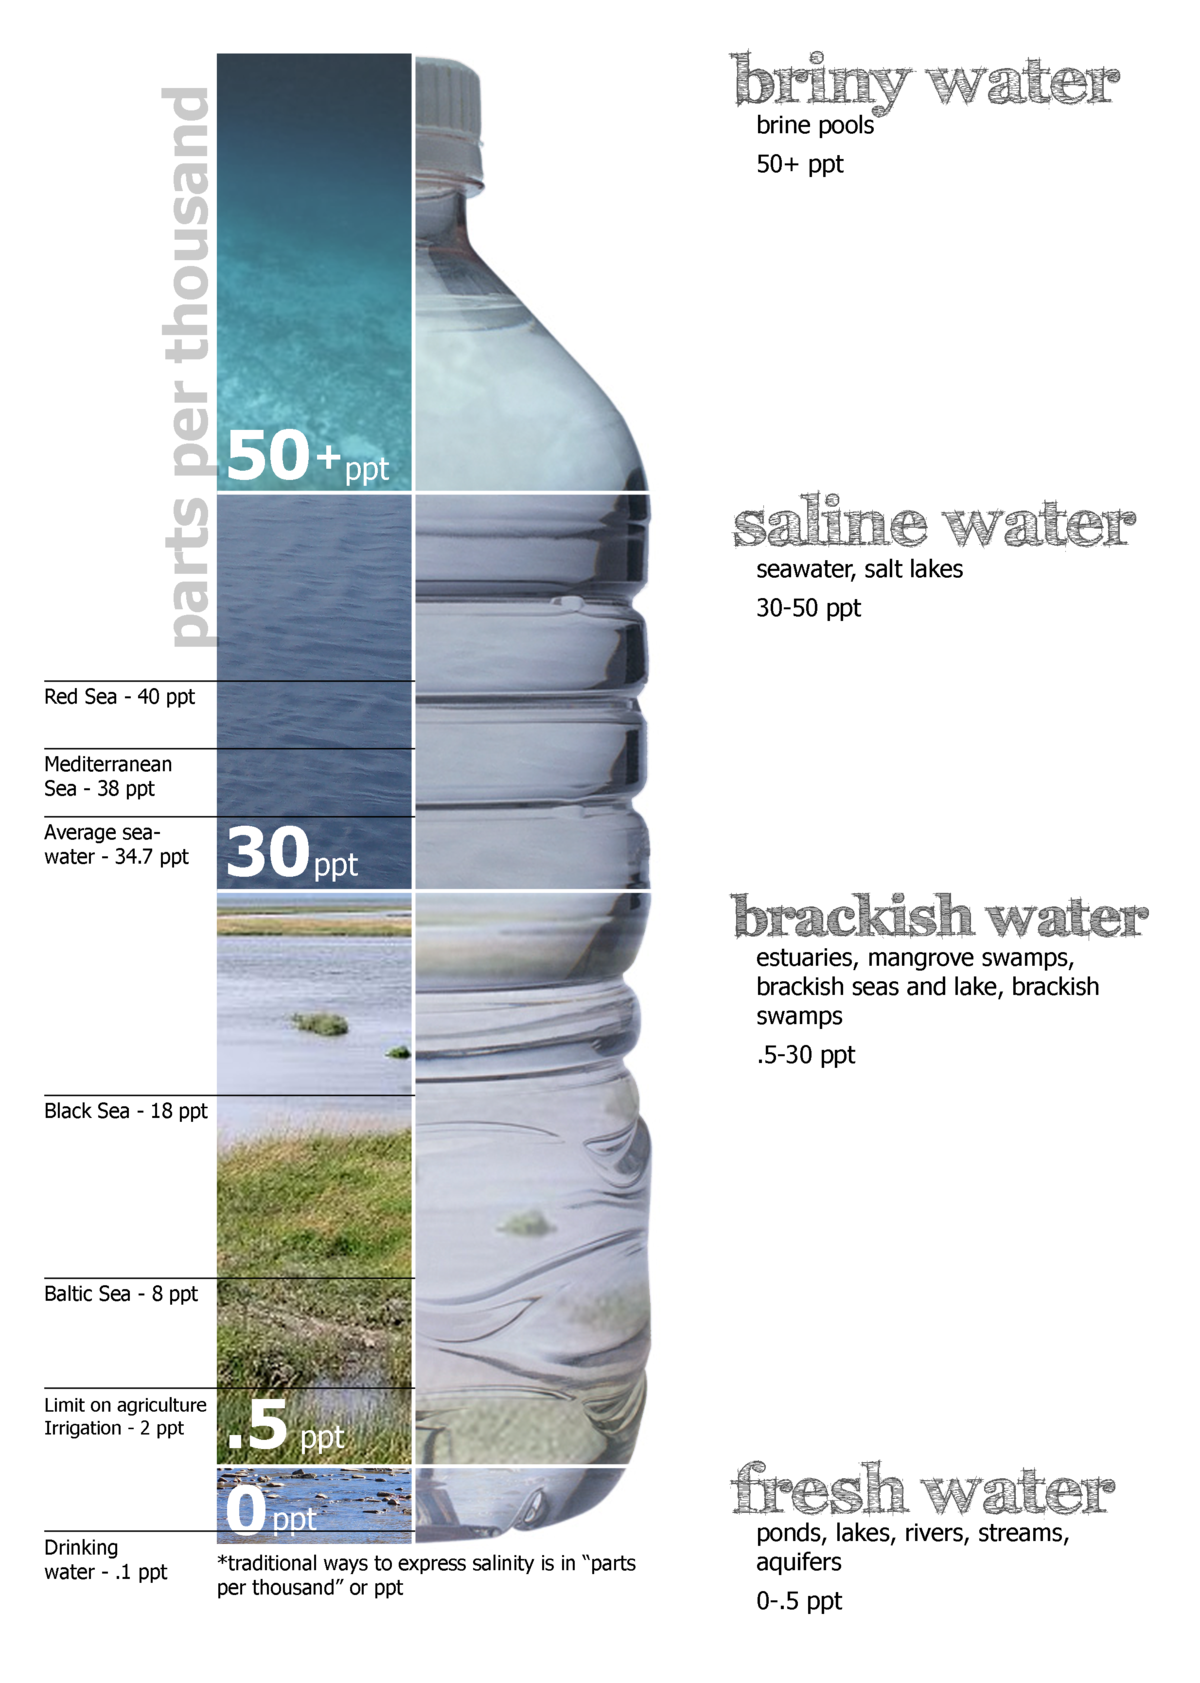
\includegraphics[width=.5\textwidth]{Water_salinity_diagram.png}
\caption{\small \sl This figure displays the differences between different water qualities.  The groundwater in Arizona qualifies as brackish \cite{USBureauofReclamation2006}.  This image is from \cite{Summerlin}}
\label{salinity}
\end{figure*}


In a multi-stage flash system, it is important to keep the temperature relatively low, no greater than 120 \degree C, in order to minimize fouling. Fouling and scaling are serious considerations for MSF systems.  Generally, fouling refers to the unwanted deposition of compounds or organic substances on the surface of a host material (membrane, heat exchanger, condenser, etc)\cite{Khayet2016}. Scaling is when a surface is entirely covered with a mineral film coating. In \cite{El-Dessouky2016} the twelve case studies range from 95 \degree C to 105 \degree C. For a more complete range of possible temperatures, this research will analyze temperatures from 80 \degree C to 120 \degree C. The largest MSF plant produces about $91,000\frac{m^3}{day}$.




\subsection{Reverse Osmosis}

Reverse osmosis is a type of electrically driven membrane desalination or filtration process. It can remove tiny particles of sizes ranging down to 50-200 daltons \cite{Pangarkar2011}. It has relatively high applied pressure values ranging between 1-5 MPa. In general, the reverse osmosis system works due to the osmotic pressure differences between salt water or brackish water and pure water. During the \ac{ro} process, salt water or brackish water is forced through membranes under pressure, separating the feedwater into a pure water stream and a stream with a high concentration of impurities.  Generally, about 4kWh is required for every cubic meter of clean water \cite{Pangarkar2011}. About 48\% of reverse osmosis systems are used with brackish water \cite{Pangarkar2011}. The largest sea water reverse osmosis desalination plant in the world is in Israel and produces about $624,000\frac{m^3}{day}$. The amount of water produced by the RO facilities in this study is significantly greater than the output of the largest facility in the world.  The goal for this research is to determine the relative potential outputs of the various configurations, not the realistic values.



\section{Methodology}
 The exergy analysis performed here will assume a simplified model of the Palo Verde Rankine power cycle, seen in figure \ref{basePC}, and compare a process heat MSF distillation system to a RO system.  First, the  \$/exergy cost of an MSF system will be evaluated using the process heat from a nuclear power plant. Then the same process will be applied to the exergy costs of the RO system, which strictly uses electricity. Traditionally an economic exergy analysis, also known as an exergonomic or thermoeconomic analysis, evaluates the most costly exergy losses in a system. In this case each of the components in the power cycle and industrial process would be evaluated based on their capital and maintenance costs as well as the specific exergy losses associated with the process.  This is commonly referred to as the \ac{speco} approach.  In this case, the motivation behind coupling with an industrial process is not minimizing the costs of generation, but instead optimizing the profit.  Evaluating the economics of the exergy losses associated with each of the components of the system does not answer the fundamental question of which system will generate the greatest profit given a fluctuating price for electricity and ever increasing price for water. The exergy losses in the RO system comes from the exergy destroyed in the pumps and is added to the exergy loss required to generate the electricity. The economic values for the system will come from the value of the electricity generated plus the value of the water generated. While the exergy analysis performedin this research does not include the capital, operations, and maintenance costs of the two systems, it does suggest what the differences are likely to be between the two systems.  It does so by demonstrating how each pump added to the RO system reduces the overall revenue per unit of exergy.

 \begin{figure*}[h!]
\centering
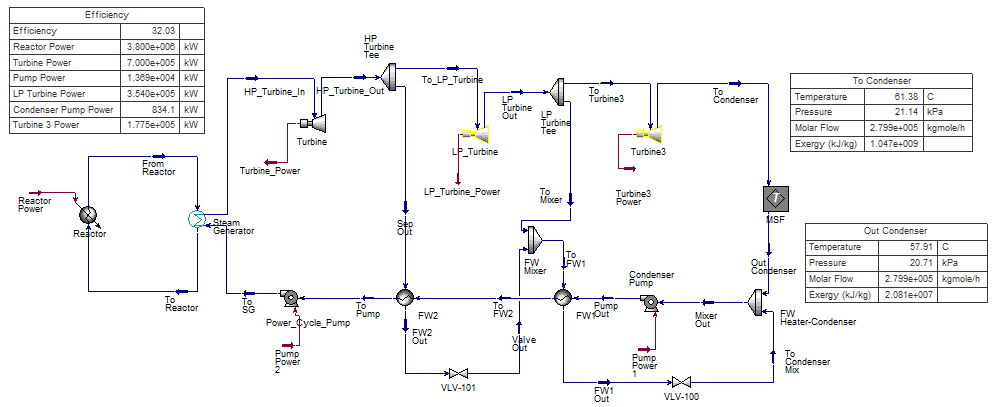
\includegraphics[width=\textwidth]{ActualPC.PNG}
\caption{\small \sl Palo Verde's simplified Rankine cycle used for this research. The overall efficiency of the system is about 32\%, which is a reasonable approximation of the Palo Verde Power cycle.  The turbines are yellow, meaning warning, because of the liquid entering the turbines.  In reality, the turbines can still function with some liquid}
 \label{basePC}
\centering
\end{figure*}

A simplified model of the \ac{pvgs} power cycle is constructed using Aspen HYSYS.  Since the goal in this research is to evaluate the differences in the water purification systems, not the exergy losses in the power cycle, the power cycle model primarily serves to demonstrate how thermally coupling a system impacts the system as a whole. While a more precise model of the \ac{pvgs} would provide more precise results, the goal of this project is to show the relative benefits of multiple water purification approaches. The overall exergy lost is the same throughout the power cycle; the losses can generate either electricity or water.

\subsection{Aspen HYSYS}

Aspen HYSYS is process simulation software used primarily by the oil and gas industry. In general, process simulation software calculates material and energy balances for a whole plant or process unit. Process simulation software can be used to size the various components in a system for the desired outcome in terms of quality and quantity of product. Aspen HYSYS calculates heat and mass balances, thermodynamic data and equilibrium conditions, sizes equipment, and can do economic optimization and dynamic simulation \cite{Oi2017}. In this model, Aspen HYSYS calculates the overall thermodynamic and mass flow values of the Palo Verde power cycle as well as the multistage flash distillation process. The thermodynamic values, such as enthalpy, entropy, temperature, and pressure can then be used to determine the exergy of the system using a User Variable in the system.

First, as can be seen in figure \ref{basePC}, determining the exergy analysis required initially building the Palo Verde power cycle using Aspen HYSYS and then coupling it to both a MSF and RO water purification systems. The configurations for the MSF and RO systems can be seen in figures \ref{MSF} and \ref{RO} respectively. After the building the model, in order to find  the \$/exergy in the power cycle and the water purification system required using a combination of user variables within Aspen HYSYS as well as spreadsheet calculations, as can be seen in Appendix B. Then, after finding the exergy values, in order to determine the optimal temperature of water required adjusting the temperature of the water sent to the heat exchanger with the MSF system.

\begin{figure*}[h!]
\centering
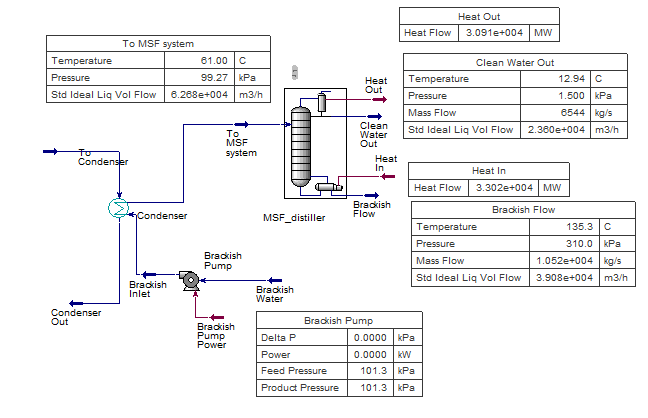
\includegraphics[width=\textwidth]{PowerCycle.PNG}
\caption{\small \sl The distillation column used to represent the multi-stage flash system along with key important metrics for the various components.}
\label{MSF}
\centering
\end{figure*}

\begin{figure*}[h!]
\centering
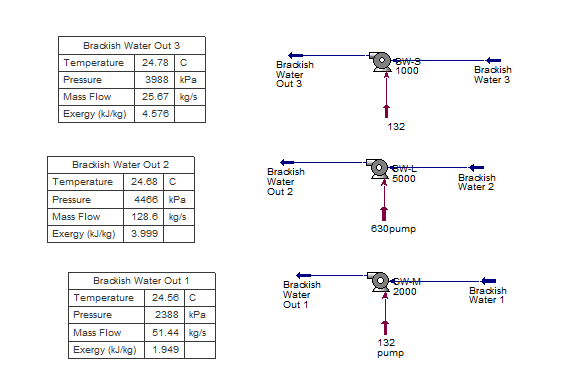
\includegraphics[width=\textwidth]{RO_3Pumps.PNG}
\caption{\small \sl The energy used for an RO system is directed almost entirely to the pumps used.  The three pumps shown here represent off-the-shelf pumps used in Reverse Osmosis systems}
\label{RO}
\centering
\end{figure*}

Doing an economic analysis evaluating the \$/exergy requires knowing the amount of product sold as well as the value of the product. The cost of water for Palo Verde in 2018 is \$130.00 per acre-foot, which comes out to about \$0.105 per cubic meter of water \cite{Brown2018}. The water Palo Verde consumes is cheap compared to the residential cost of water in Tucson which was about \$1.42 per cubic meter in 2017\cite{CityofTucson2017}. The best value available for the wholesale value of Palo Verde's electricity is from 2007 at 6.33 cents per kWh, which is equal to about 8 cents per kWh in 2018 dollars including inflation over the past 11 years. The actual value of the electricity varies over a day depending on the supply of electricity and grid demand. The highest wholesale price paid per MWh in the Palo Verde Southwest price hub was \$165.  The lowest wholesale price paid per MWh in the Palo Verde Southwest price hub was \$13.50 \cite{EIA2017}.  The \$80 per MWh price assumed in this research is on the high side, but still within the range.  The actual wholesale price of electricity for Palo Verde is confidential information, so the price values are approximations.  In Arizona's case, the value of the electricity over the course of a day is largely influenced by the amount of solar supply available to the grid from both Arizona and California. The fluctuation in power demand for \ac{aps} will be taken into consideration using \ac{raven} to generate demand data for a generic day in each season.

\subsection{Fluctuating Electricity Output}

The definition of a regulating and supplemental reserve of electricity differs depending on the region and \ac{iso}.  The Independent Electricity System Operator (IESO), which manages most of Ontario, Canada's grid maintains that spinning reserve, such as nuclear plants, to be considered operating reserve, or 10-minute spinning, must make energy available within 10 minutes of the contingency so that the supply matches the demand\cite{NERC2014}. NPPs traditionally are unable to fulfill a role as regulating or supplemental reserve because of the inability to ramp to full power quickly.  With an MSF system, the NPP still may be unable to switch the process heat fast enough to meet the IESO's definition. The European Utility Requirements require that an NPP be capable of daily load cycling operation between 50\% and 100\%. The European pressurized water reactor must satisfy maneuverability requirements, including being able to have planned variations in energy output between 25\% and 100\% \cite{Nuclear2011}. There are several nuclear power plants which are already manipulating the amount of load they send to the grid.  Energy Northwest is reducing the amount of load it sends to the grid to 80\% of capacity when there is too much electricity on the grid and the price of electricity is low.  Duke Energy is currently evaluating how to reduce their nuclear output to the grid, also establishing a minimum of 80\% of rated capacity \cite{siphers}.  Since the standards are significantly different in the United States as compared to Europe, smaller fluctuations ranging from between 5\% and 20\% will also be evaluated for each of the cases.For this research, the water purification systems will be evaluated at 5\%, 10\%, 15\%, 20\%, 25\%, 50\%, 75\%, and 100\% of the electricity from the reactor.

\subsection{Drinking Water Standards}
Water quality standards must be met to ensure the water produced by the purification process is of high enough quality to use in Palo Verde's power cycle as well as to sell to the public. The main consideration for the water purification system, especially if the water is planned for sale to the public, is that the water must meet the standards established by the Safe Drinking Water Act of 1974. While commercial nuclear power plants dedicate a lot of resources to water chemistry and have very high standards for the water used in the plant, the standard used for this research will be that set for public consumption. The Safe Drinking Water Act of 1974 gives the \ac{epa} the authority to determine drinking water standards. The EPA sets standards on over ninety contaminants in drinking water. The drinking water contaminants fall into the broad categories of microorganisms, disinfection byproducts, disinfectants, inorganic chemicals, organic chemicals, and radionuclides \cite{USEPA}. The make up of Arizona groundwater can be found in table \ref{ArizonaWater}.  None of the contaminants found in Arizona groundwater are regulated by the Safe Drinking Water Act or are covered by the EPA's secondary drinking water standards \cite{USEPA}. The only overlap between the contaminants regulated by the EPA for taste and aesthetic concerns and those found in Arizona groundwater is maintaining the total dissolved solids at 500 mg/L or below. For this research, the water is assumed to be comprised of a more brackish composition than that found in table \ref{ArizonaWater}. The contaminants have been increased nine fold in the composition used in the Aspen HYSYS model, as can be seen in table \ref{ModelComp}.  In some cases, the independent materials found in the brackish ground water were unavailable in the Aspen library.  As a result, the model includes combined molecules, such as sodium sulfate and sodium nitrate to most closely proportionally match the composition found in the groundwater.  Combining these molecules may result in some difference in the overall composition and the energy it takes to remove the particulates. The end product is clean water, with the model composition displaying 100\% water.

\begin{table}[h!]
\centering
\caption{Mole Composition of Brackish Groundwater Assumed in Aspen-HYSYS model}
\begin{tabular}{|l|l|}
\hline
\multicolumn{1}{|c|}{\textbf{Material}}                   & \multicolumn{1}{c|}{\textbf{Mole Percent}} \\ \hline
Calcium & 1.3E-1 \\ \hline
Magnesium  & 9E-2\\ \hline
Sodium  & 5E-1 \\ \hline
Sodium-Sulfate & 1.7E-1 \\ \hline
Sodium-Nitrate & 9E-2 \\ \hline
Barium & 1E-2 \\ \hline
Water & 99.0  \\ \hline
\end{tabular}
\label{ModelComp}
\end{table}

\section{Palo Verde Power Cycle}

Much of the information on the design and functioning of Palo Verde's power cycle can be found in the \ac{ufsar}, as can be seen in tables \ref{coreValues} and \ref{PowerValues} made publicly available for all nuclear power plants by the \ac{nrc}. Some of the key values taken from Palo Verde's \ac{ufsar} are displayed in tables \ref{coreValues} and \ref{PowerValues}.  The second value represents the converted value into the units used in the model of this thesis.  The key difference between the model values and the Main Steam Flow Power Cycle Values is the mass flow is significantly less for the model 1616- $\frac{kg}{s}$ compared to 2200 $\frac{kg}{s}$. The mass flow value is solved for in the model. As the thermodynamic values taken for this research are specific values that do not include the mass flow, the findings should be relevant to any mass flow. Overall, while the simplified Palo Verde power cycle does not precisely model the actual power plant, it has enough similarities to suggest some trends via the exergy analysis. Since not all of the components are included in the model, the lower mass flow calculated is to be expected.

\begin{table}[h!]
\centering
\caption{Palo Verde Reactor Core Thermohydraulic Values. The first units given in the Value Given in FSAR column are the actual values found in the FSAR, while the second are the converted values into those used in the model.}

\begin{tabular}{|l|l|l|}
\hline
\textbf{Reactor Core Values} & \textbf{Value Given in FSAR} & \textbf{Value in Model}        \\ \hline
Reactor Outlet Temperature   & 653 \degree F, 345\degree C & 345 \degree C   \\ \hline
Reactor Inlet Temperature    & 568 \degree F, 297.8 \degree C &  297\degree C\\ \hline
Mass Flow                    & $164.0x10^6\frac{lb}{hr}$    & $20663.6\frac{kg}{s}$          \\ \hline
Pressure                     & 2250 psia, 15.513 MPa                    &  15.51 MPa                    \\ \hline
Power Generation             & 3990 MWt                     & 3990 MWt                       \\ \hline
\end{tabular}
\label{coreValues}
\end{table}


\begin{table}[h!]
\centering
\caption{Palo Verde Main Steam Flow Power Cycle.}
\label{PowerValues}
\begin{tabular}{|l|l|l|}
\hline
\textbf{Power Cycle Values} & \textbf{Value Given in FSAR}  & \textbf{Values in Model}          \\ \hline
Steam Temperature at HX     & 552.9 \degree F (289.4 \degree C) &   289.4 \degree C                 \\ \hline
Mass Flow                   & $17.2-18.1x10^6\frac{lb}{hr}$ ($2154.56-2280.56 \frac{kg}{sec}$) & 1616 $\frac{kg}{sec}$ \\ \hline
Pressure & 1070 psia (7.377 MPa)  &   7.377 MPa                     \\ \hline
\end{tabular}
\label{PowerValues}
\end{table}

There are two MSF model configurations included in this analysis.  One of the configurations, as seen in figure \ref{MSF_condense},  draws water from the end of the power cycle.  As the Palo Verde Power Plant would want to minimize impact to the thermal hydraulics of the system, using the condenser and switching to passing groundwater through the system would allow for use of existing infrastructure. The second configuration, shown in figure \ref{MSF_SG}, allows for a more efficient system that draws water straight from the steam generator at very high temperatures. Since the efficiency of the ideal Carnot cycle is very dependent on the change in temperature through the cycle, drawing water from the steam generator allows for a greater drop in temperature throughout the cycle.  When taking a percentage of the water at the beginning of the power cycle, the water leaving the last turbine does not have to be a minimum of 80\degree C for the \ac{msf} system.  Also, water at 289.4\degree C can heat a lot of water at 24.44\degree C to 80\degree C. The second configuration allows for allocating different mass flows to be sent to the MSF as opposed to different temperatures of water, as is the case when using the condenser as a heat exchanger for the MSF system.

\begin{figure*}[h!]
\centering
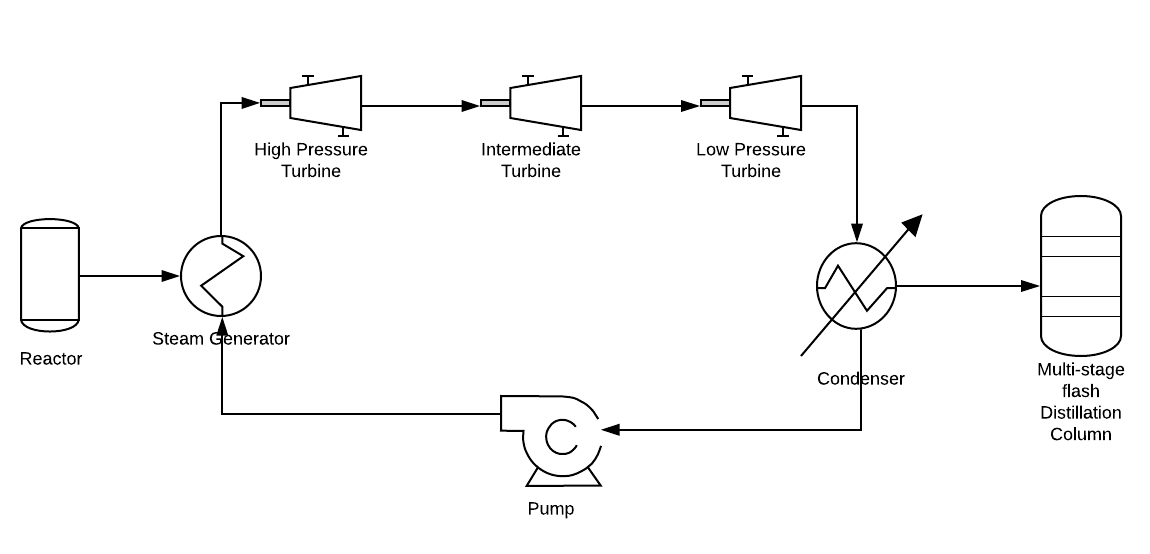
\includegraphics[width=.8\textwidth]{MSF_condense.png}
\caption{\small \sl This simplified drawing shows the main components of the power cycle including how the multistage flash distillation system is heated through the condenser}
 \label{MSF_condense}
\centering
\end{figure*}

\begin{figure*}[h!]
\centering
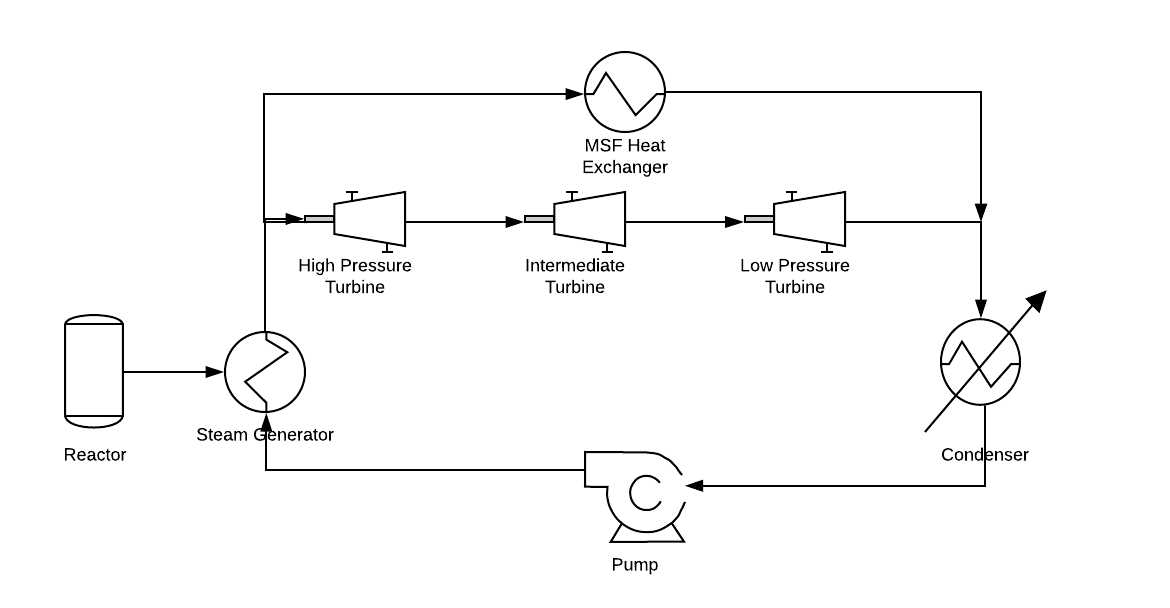
\includegraphics[width=.8\textwidth]{MSF_lucidchart.png}
\caption{\small \sl This simplified drawing shows the main components of the power cycle including how the multistage flash distillation system draws water just after the steam generator}
 \label{MSF_SG}
\centering
\end{figure*}
\clearpage

\subsection{Assumptions}

Given the information above, the assumptions for both the \ac{msf} and \ac{ro} Aspen HYSYS models are:
\begin{enumerate}
\item The temperature of the brackish groundwater entering the system is 76 \degree F or 24.44 \degree C, the low end of the temperature range for the water currently used to cool the system \cite{Brown2018}. Groundwater would be colder, but sitting in a pool above ground would raise the temperature. The assumption of the water being at the low end of what currently flows through the condenser allows an analysis of using the groundwater and also allows for a fair comparison of the MSF and RO systems using the most realistic value for both.
\item The reactor power, as given in the FSAR, is 3990 MWth.
\item The temperatures for the MSF distillation unit range from 80 \degree C to 120 \degree C. Since the 80\degree C water generated the most water in each circumstance, only the 80\degree C model is discussed.
\item The composition of the water is shown in \ref{ModelComp}.
\item There is a 2\% pressure drop across all heat exchangers.
\item The turbines in the Palo Verde power cycle have a 90\% adiabatic efficiency.
\item The pumps have a 90\% adiabatic efficiency.
\item The fluid package used for the power cycle is Peng-Robinson, which is the fluids package with the largest applicable range for temperature and pressure.
\item The fluid package used for the brackish water is Aspen's Electrolyte Non-Random Two-Liquid (NRTL). This fluid package is especially good for modeling all of the various components in the brackish feedwater composition.
\item The power cycle is much simplified in order to show the clear impacts of the different water purification techniques as opposed to emphasizing the power cycle itself.
\end{enumerate}

The assumptions for the MSF Aspen HYSYS models are:

\begin{enumerate}
\item There are twenty one stages in the MSF distillation system \cite{Bodalal2010}.
\item The mass flow through the distillation system is the dependent variable while the temperature of the water sent to the unit and the pressure generated from the brackish water pump are the independent variables for the MSF system.
\item The reactor power and electricity produced are independent variables.
\item The temperature of the water sent to the condenser is an independent variable.
\item The pump power is a dependent variable.
\item The electric power generated is an independent variable.
\item The amount of water generated and the electricity generated are the dependent variables depending on the desired temperature of water sent to the condenser.
\end{enumerate}

The assumptions for the RO Aspen HYSYS model are:

\begin{enumerate}
\item The efficiency of the pumps range from 70\% to 80\% depending on the specifics of the expected pressure and water outflow provided by the company, the specifics of which can be seen in Appendix \ref{Appendix:pumps}.
\end{enumerate}

The economic assumptions for all Aspen HYSYS models are:
\begin{enumerate}
\item The cost of water for Palo Verde Generating Station is \$130 per acre foot \cite{Brown2018}
\item The wholesale price which Palo Verde can sell electricity to the grid is \$.08 per kWh.
\end{enumerate}

The simplified Aspen HYSYS model for the normal 100\% electricity production power cycle includes one high pressure and two low pressure turbines.  The three separate turbines can be taken offline independently to send higher temperature water to the MSF system. The exergy analysis performed here is different than most economic exergy analyses in that it considers the revenue from each product, not the cost. Generally, exergy analyses consider the costs of each of the various systems to see where the greatest cost to exergy losses exists. For example, if exergy losses at a pump cost a lot to the system as a whole as compared to exergy losses at a heat exchanger, the pump should be replaced first.  As the prices for the various products are more readily found than the cost of generating the electricity or the steam, the revenue is evaluated here.  While a revenue based \ac{speco} approach is currently in development, one of the built-in assumptions of the model currently is the revenue associated with any given unit of exergy will be the same no matter if the heat is used to generate electricity or a secondary produce \cite{Paulus2006}.  In the case of a system that generates multiple products, such as the system evaluated in this thesis, and uses exergy that would otherwise go unused, there is a difference in the exergy value at different locations in the system. Therefore the approach employed in this research is very basic, looking strictly at the revenue generated from the products and the exergy generated by the reactor. Calculation of the \$/exergy values for this analysis the following calculations were applied:

Using equation \ref{electricity}, the electricity revenue is calculated by multiplying the electricity produced by the system in MW by the wholesale electricity price per MWh, assumed here to be \$80 per MWh:
\begin{equation}
Electricity\hspace{.175cm} Revenue=MW_{out}*\frac{\$80}{MWh}=\frac{\$}{hr}
\label{electricity}
\end{equation}

The water revenue is then calculated using equation \ref{water}, which multiplies the water produced by the system by the wholesale value of water to Palo Verde Generating Station, $\frac{\$0.105}{m^3}$:
\begin{equation}
Water\hspace{.2cm} Revenue=\frac{m^3_{out}}{hr}*\frac{\$.105}{m^3}=\frac{\$}{hr}
\label{water}
\end{equation}

Equation \cite{revenueX} is then applied to find the \$/exergy destroyed:
\begin{equation}
\frac{\$}{Exergy\hspace{.175cm}destroyed}=\frac{Electricity \hspace{.175cm} Revenue+ Water \hspace{.2cm} Revenue} {Total\hspace{.175cm}Exergy\hspace{.175cm}Destroyed\hspace{.175cm}in\hspace{.175cm}Power\hspace{.175cm}Cycle}
\label{revenueX}
\end{equation}

Generally, an exergy analysis evaluates the cost per unit of specific exergy.  Overall it analyzes how much is spent in generating every unit of exergy and therefore how much is worth spending to enhance the exergy efficiency through other steps, such as purchasing more efficient pumps, condensers, or turbines.  The initial exergy analysis in this research attempts to look purely at the revenue per unit of exergy.  Since the value of the electricity and water are already known, the approach of evaluating the overall revenue establishes an initial means of analyzing the system. The exergy analysis finds the exergy generated by the reactor and analyzes which coupled water purification design uses that exergy to generate the greatest overall revenue.  This is a simple analysis which does not include the operations, maintenance, or capital cost.  It simply determines how the exergy can be allocated to result in the greatest overall revenue.


\section{Results}

The results of this study focus on answering questions about three possible beneficial areas from coupling Palo Verde to a water purification system. The benefits include 1) varying the electricity output to the grid, 2) optimizing the value of the exergy lost in the system, and 3) providing reliable and reasonably priced water to Palo Verde.  The results are organized to focus on these three considerations.


\subsection{Flexibility}
The ability of a system to operate flexibly is of growing significance and value. As greater variable electricity sources are added to the grid, other generation sources will need to change their output to the grid in response. A more thorough analysis of the flexibility requirements for Palo Verde is provided in section 3.5. There is a value in sending various loads to the water purification process for different points in the day as the power needs of the grid vary. To do a parametric study of the ability for the RO system and the MSF systems to take the different amounts of load, the model is evaluated first at 5\%, 10\%, 15\%, and 20\% and then at 25\%, 50\%, 75\%, and 100\% of the electricity allocated to the purification system with the exception of the MSF system coupled at the condenser. This configuration is unable to reduce to 5\% output due to meeting the minimum heat requirement of 80\degree C requiring more than 5\% of the energy from the power cycle. The lower level load allocation to the water purification facilities is more realistic both based on the size of the water purification facilities and on the overall impact to the nuclear power plant.

This thesis does not include a quantitative study of the ability of the two water purification techniques to start and stop, but the research literature suggests the reverse osmosis systems are easier to run in a dynamic fashion.  The MSF system requires careful maintenance between the power generation and water generation processes.  There is a small range of temperatures within which the MSF unit can operate.  If performed improperly, the MSF unit could automatically trip off \cite{Radif}.  The RO systems, being essentially a large number of pumps forcing water through membranes, are able to start and stop while producing the same quality of water.  Both systems are able to start and stop.  In the AHP analysis, desalination ranked highest in flexibility. While this is an imperfect measure, it does suggest that the flexibility is a benefit of desalination.

Tables \ref{SGLF} through \ref{SW-L} display the overall \$/exergy values as well as how much electricity and water were generated hourly. The exergy destruction in the power cycle is the only exergy taken into consideration. The tables show which system generates the most revenue for the exergy created by the reactor.  The greatest overall  \$/exergy value is the SW-L 630  reverse osmosis system at $\frac{\$97.93}{\frac{kJ}{kg}}$  This is notably less than the \$/exergy of solely generating electricity of $\frac{\$100.77}{\frac{kJ}{kg}}$ at the given prices. The reverse osmosis systems have both greater revenue and a greater exergy value than the MSF systems.  The MSF configuration connected directly after the steam generator has a significantly greater \$/exergy value than the one coupled at the condenser. The MSF unit coupled at the condenser can generate a lot of water with lower levels of power, but the RO unit linearly outputs water.

The largest reverse osmosis plant in the world, the Sorek plant in Israel by \ac{ide}, produces about $627,000 \frac{m^3}{day}$, or about $26,000\frac{m^3}{hr}$ of water \cite{Talbot2015}. The largest MSF distillation system in the world produces approximately $728,000\frac{m^3}{day}$, or about $30,300\frac{m^3}{hr}$.  The values shown in the results tables greater than the 20\% allocation are significantly greater than the output of the largest water purification systems in the world, which is unreasonable. The number of pumps required for sending large quantities of electricity to the reverse osmosis system are not reasonable. Similarly, the size of the MSF unit would need to be enormous to use large quantities of heat from the reactor.  The reason for including the deep load following percent reduction is to show how the two systems compare based on revenue. The results are there to demonstrate the differences between the different configurations. The capital costs would be too great to build configurations sufficiently large to operate flexibly above about 5\% of one of Palo Verde's reactors.

\begin{table}[h!]
\centering
\caption{Load following outcomes using the thermally coupled MSF distillation system drawing heat directly after the steam generator at smaller interval load reductions assuming a 20\% reduction limit}
\label{SGLF}
\begin{tabular}{|l|l|l|l|l|l|l|}
\hline
\multicolumn{1}{|c|}{\textbf{\begin{tabular}[c]{@{}c@{}}Load\\  Following\\ Percent \\ Reduction\end{tabular}}} & \multicolumn{1}{c|}{\textbf{\begin{tabular}[c]{@{}c@{}}Percent \\ Water\\ Split\end{tabular}}} & \textbf{\begin{tabular}[c]{@{}l@{}}Volume\\ Flow Out\\ $\frac{m^3}{hr}$\end{tabular}} & \textbf{\begin{tabular}[c]{@{}l@{}}Power\\ MWe\end{tabular}} & \textbf{\begin{tabular}[c]{@{}l@{}}Hourly \\ Total\\ Revenue\\ (\$/hr)\end{tabular}} & \textbf{\$/exergy} \\ \hline
5\%   & 0.988   & 607.5  & 1244.86    & 99652.75 & 96.93            \\ \hline
10\%  & 0.9403  & 3003 & 1178.61 & 94604.09  & 89.65            \\ \hline
15\%  & 0.901 & 4920  & 1134.83   & 91303.24  & 88.00  \\ \hline
20\%   & 0.86  & 7077 & 1044   & 84263.09  &81.62 \\ \hline
\end{tabular}
\label{SGLF}
\end{table}

\begin{table}[h!]
\centering
\caption{Load following outcomes using the thermally coupled MSF distillation system drawing heat directly after the steam generator at the load reduction levels required for European reactors \cite{Nuclear2011}.}
\begin{tabular}{|l|l|l|l|l|l|l|}
\hline
\multicolumn{1}{|c|}{\textbf{\begin{tabular}[c]{@{}c@{}}Load\\  Following\\ Percent \\ Reduction\end{tabular}}} & \multicolumn{1}{c|}{\textbf{\begin{tabular}[c]{@{}c@{}}Percent \\ Water\\ Split\end{tabular}}} & \textbf{\begin{tabular}[c]{@{}l@{}}Volume\\ Flow Out\\ $\frac{m^3}{hr}$\end{tabular}} & \textbf{\begin{tabular}[c]{@{}l@{}}Power\\ MWe\end{tabular}} & \textbf{\begin{tabular}[c]{@{}l@{}}Hourly \\ Total\\ Revenue\\ (\$/hr)\end{tabular}} & \textbf{\$/exergy} \\ \hline
25\%  & 0.85	& 7396 &	979.2 &79112.581 &	75.86 \\ \hline
50\% & 0.68 & 15400 &	654.8 &	54001 &	51.17
  \\ \hline
75\% &  0.39 &	28540 &	327.5 &		29196.7 &	27.34\\ \hline
100\%  & 0  &  42450 &	0 &	 4457.25 &	4.18 \\ \hline

\end{tabular}
\label{LoadFollowSG}
\end{table}

\begin{table}[h!]
\centering
\caption{Load following outcomes using the thermally coupled MSF distillation system with the heat sent to the condenser at various load reduction levels assuming a 20\% reduction floor. The load following percent is controlled by sending varying amounts of heat to the condenser leading to the \ac{msf}.}

\begin{tabular}{|l|l|l|l|l|}
\hline
\multicolumn{1}{|c|}{\textbf{\begin{tabular}[c]{@{}c@{}}Load\\  Following\\ Percent \\ Reduction\end{tabular}}} & \textbf{\begin{tabular}[c]{@{}l@{}}Volume\\ Flow Out\\ $\frac{m^3}{hr}$\end{tabular}} & \textbf{\begin{tabular}[c]{@{}l@{}}Power\\ MWe\end{tabular}} & \textbf{\begin{tabular}[c]{@{}l@{}}Hourly \\ Total\\ Revenue\\ (\$/hr)\end{tabular}} & \textbf{\$/exergy} \\ \hline
10\% & 29940 &	1178.631 &	97434.18 &	92.21
 \\ \hline
15\%  & 31370 &	1134.28 &	94036.17 &	89.65
 \\ \hline
20\%  &  31510 & 1044	& 	86828.55 &	82.23  \\ \hline
\end{tabular}
\label{LowCondLF}
\end{table}


\begin{table}[h!]
\centering
\caption{Load following outcomes using the thermally coupled MSF distillation system with the heat sent to the condenser at the  load reduction levels required for European reactors \cite{Nuclear2011}. The load following percent is controlled by sending varying amounts of heat to the condenser leading to the \ac{msf}.}

\begin{tabular}{|l|l|l|l|l|}
\hline
\multicolumn{1}{|c|}{\textbf{\begin{tabular}[c]{@{}c@{}}Load\\  Following\\ Percent \\ Reduction\end{tabular}}} & \textbf{\begin{tabular}[c]{@{}l@{}}Volume\\ Flow Out\\ $\frac{m^3}{hr}$\end{tabular}} & \textbf{\begin{tabular}[c]{@{}l@{}}Power\\ MWe\end{tabular}} & \textbf{\begin{tabular}[c]{@{}l@{}}Hourly \\ Total\\ Revenue\\ (\$/hr)\end{tabular}} & \textbf{\$/exergy} \\ \hline
25\%  &  32160 & 979.2	& 	81712.8 &	77.39  \\ \hline
50\%   &  35480 &	654.8 &		56109.4 &	53.10  \\ \hline
75\%  & 38960 &	327.5 &	30290.8 &	28.88
 \\ \hline
100\%  &  42450 &	0 &		4457.25 &	4.18   \\ \hline
\end{tabular}
\label{LoadFollow}
\end{table}


\begin{table}[h!]
\centering
\caption{Exergy Analysis of the IDE-Progreen SW-S 132 kW pump assuming a 20\% reduction limit}
\begin{tabular}{|l|l|l|l|l|l|}
\hline
\multicolumn{1}{|c|}{\textbf{\begin{tabular}[c]{@{}c@{}}Load\\  Following\\ Percent \\ Reduction\end{tabular}}} & \multicolumn{1}{c|}{\textbf{\begin{tabular}[c]{@{}c@{}}Number of\\ Pumps\end{tabular}}} & \textbf{\begin{tabular}[c]{@{}l@{}}Volume\\ Flow Out\\ $\frac{m^3}{hr}$\end{tabular}} & \textbf{\begin{tabular}[c]{@{}l@{}}Power\\ MWe\end{tabular}} & \textbf{\begin{tabular}[c]{@{}l@{}}Hourly \\ Total\\ Revenue\\ (\$/hr)\end{tabular}} & \textbf{\$/exergy} \\ \hline
5\% &	497 &	20729.87 &	1244.396 & 101728.32	 &	97.83
 \\ \hline
10\% &	993 &	41418.03 &	1178.92 &	98662.81 &	94.88
 \\ \hline
15\% &	1489 &	62106.19 &	1113.452 &	95597.31 &	91.93
 \\ \hline
20\% &	1985 &	82794.35 &	1047.98 &	92531.81  &	 88.98
 \\ \hline
\end{tabular}
\label{SW-S_floor}
\end{table}



\begin{table}[h!]
\centering
\caption{Exergy Analysis of the IDE-Progreen SW-S 132 kW pump}
\begin{tabular}{|l|l|l|l|l|l|}
\hline
\multicolumn{1}{|c|}{\textbf{\begin{tabular}[c]{@{}c@{}}Load\\  Following\\ Percent \\ Reduction\end{tabular}}} & \multicolumn{1}{c|}{\textbf{\begin{tabular}[c]{@{}c@{}}Number of\\ Pumps\end{tabular}}} & \textbf{\begin{tabular}[c]{@{}l@{}}Volume\\ Flow Out\\ $\frac{m^3}{hr}$\end{tabular}} & \textbf{\begin{tabular}[c]{@{}l@{}}Power\\ MWe\end{tabular}} & \textbf{\begin{tabular}[c]{@{}l@{}}Hourly \\ Total\\ Revenue\\ (\$/hr)\end{tabular}} & \textbf{\$/exergy} \\ \hline
25\% & 2482 & 103524.22  & 982.376 & 89460.12   & 86.03 \\ \hline
50\%  & 4963  &207006.73  & 654.884 & 74126.43 & 71.28   \\ \hline
75\%   & 7444    &310489.24  & 327.392  & 58792.73 & 56.54  \\ \hline
100\% & 9925 &  413971.75  & 0  & 43467.03  & 41.80 \\ \hline
\end{tabular}
\label{SW-S}
\end{table}

\begin{table}[h!]
\centering
\caption{Exergy Analysis of the IDE-Progreen SW-L 630 kW pump assuming a 20\% reduction limit}

\begin{tabular}{|l|l|l|l|l|l|}
\hline
\multicolumn{1}{|c|}{\textbf{\begin{tabular}[c]{@{}c@{}}Load\\  Following\\ Percent \\ Reduction\end{tabular}}} & \multicolumn{1}{c|}{\textbf{\begin{tabular}[c]{@{}c@{}}Number of\\ Pumps\end{tabular}}} & \textbf{\begin{tabular}[c]{@{}l@{}}Volume\\ Flow Out\\ $\frac{m^3}{hr}$\end{tabular}} & \textbf{\begin{tabular}[c]{@{}l@{}}Power\\ MWe\end{tabular}} & \textbf{\begin{tabular}[c]{@{}l@{}}Hourly \\ Total\\ Revenue\\ (\$/hr)\end{tabular}} & \textbf{\$/exergy} \\ \hline
5\% &	104 &	21673.6 &	1244.48 &	101834.128 &	97.93
 \\ \hline
10\% &	208 &	43347.2 &	1178.96 &	98868.26 &	95.07
 \\ \hline
15\% &	312	& 65020.8 &	1113.44 &	95902.384 &	92.22
 \\ \hline
20\% &	416 &	86694.4 &	1047.92 &	92936.512 &	89.37

 \\ \hline
\end{tabular}
\label{SW-L_floor}
\end{table}


\begin{table}[h!]
\centering
\caption{Exergy Analysis of the IDE-Progreen SW-L 630 kW pump}
\begin{tabular}{|l|l|l|l|l|l|}
\hline
\multicolumn{1}{|c|}{\textbf{\begin{tabular}[c]{@{}c@{}}Load\\  Following\\ Percent \\ Reduction\end{tabular}}} & \multicolumn{1}{c|}{\textbf{\begin{tabular}[c]{@{}c@{}}Number of\\ Pumps\end{tabular}}} & \textbf{\begin{tabular}[c]{@{}l@{}}Volume\\ Flow Out\\ $\frac{m^3}{hr}$\end{tabular}} & \textbf{\begin{tabular}[c]{@{}l@{}}Power\\ MWe\end{tabular}} & \textbf{\begin{tabular}[c]{@{}l@{}}Hourly \\ Total\\ Revenue\\ (\$/hr)\end{tabular}} & \textbf{\$/exergy} \\ \hline
25\%  &520  & 108316 & 982.4  & 89965.18   & 86.51 \\ \hline
50\%  & 1040  & 216632 & 629.22 & 73083.96 & 70.28  \\ \hline
75\% &1560  & 324948 & 327.2 & 60295.54 & 57.98 \\ \hline
100\% & 2080 & 433264 & 0  & 45530.52 & 43.78 \\ \hline
\end{tabular}
\label{SW-L}
\end{table}

\newpage
\subsubsection{Price to Switch Commodities}

Tables \ref{CostElectricity} and \ref{CostWater} provide some operations insight behind tables \ref{SGLF}-\ref{SW-L}.  The tables display at what price for electricity, \ref{CostElectricity}, and for water \ref{CostWater}, the owner should switch to generating water as well as electricity. The price values were determined by changing the price for the electricity and water to the point where the alternative configuration with water generation had a greater \$/exergy value the basic power cycle with no water generation.   For the RO systems, it makes sense to start producing water at the relatively high value of electricity of approximately  \$33.10/MWh and \$34.75/MWh respectively.  The high price suggests that much of the time it would make more sense in terms of revenue generation to allocate electricity to water production. Similarly for the RO systems, the price of water, while needing to double, is well within the range of likely water prices at about $\frac{0.254}{m^3}$ and $\frac{0.242}{m^3}$ respectively. The price of electricity would need to decrease substantially or the price of water increase substantially for the MSF configurations to make sense. Once again, it is important to note the capital, operations, and maintenance costs will play a substantial role in the overall decision making and profitability.

\begin{table}[h!]
\centering
\caption{Analysis of when the \$/Exergy value of the various configurations is greater than a system strictly generating electricity by fluctuating the price of electricity}
\begin{tabular}{|l|l|l|l|l|l|l|}
\hline
\textbf{Configuration}     & \multicolumn{1}{c|}{\textbf{\begin{tabular}[c]{@{}c@{}}Percent\\   Allocation\end{tabular}}} & \multicolumn{1}{c|}{\textbf{\begin{tabular}[c]{@{}c@{}}Electricity \\Price\end{tabular}}} & \multicolumn{1}{c|}{\textbf{\begin{tabular}[c]{@{}c@{}}Water \\Price\end{tabular}}} & \textbf{\textbf{\begin{tabular}[c]{@{}c@{}}Total\\Revenue\end{tabular}}} & \textbf{\$/Exergy} & \textbf{\begin{tabular}[c]{@{}c@{}}No Water\\ \$/Exergy\end{tabular}} \\ \hline
\textbf{100\% Electricity} & 0                                                                                            & 80                                              & 0.105                                     & 104800                 & 100.77             & 100.77                               \\ \hline
\textbf{Condenser} & 10\%   & 20.50   & 0.105 & 27305.64  & 25.88 & 100.77\\ \hline
\textbf{Condenser}         & 15\%  & 17.35                                           & 0.105                                     & 22973.59               & 21.9               & 21.85                                \\ \hline
\textbf{Condenser}         & 20\%                                                                                         & 11.5                                            & 0.105                                     & 15314.55               & 14.5               & 14.49                                \\ \hline
SG                         & 5\%                                                                                          & 1.2                                             & 0.105                                     & 3389.7                 & 1.51               & 1.51                                 \\ \hline
\textbf{SG}                & 10\%                                                                                         & 2.05                                            & 0.105                                     & 3668.07                & 2.59               & 2.58                                 \\ \hline
\textbf{SG}                & 15\%                                                                                         & 3                                               & 0.105                                     & 3979.2                 & 3.78               & 3.78                                 \\ \hline
\textbf{SG}                & 20\%                                                                                         & 2.9                                             & 0.105                                     & 3770.69                & 3.65               & 3.65                                 \\ \hline
\textbf{RO-132}            & 5\%                                                                                          & 33.1                                            & 0.105                                     & 43366.14               & 41.7               & 41.69                                \\ \hline
\textbf{RO-132}            & 10\%                                                                                         & 33.1                                            & 0.105                                     & 43371.28               & 41.7               & 41.69                                \\ \hline
\textbf{RO-132}            & 15\%                                                                                         & 33.1                                            & 0.105                                     & 43376.41               & 41.7               & 41.69                                \\ \hline
\textbf{RO-132}            & 20\%                                                                                         & 33.1                                            & 0.105                                     & 43381.54               & 41.7               & 41.69                                \\ \hline
\textbf{RO-630}            & 5\%                                                                                          & 34.75                                           & 0.105                                     & 45521.41               & 43.77              & 43.77                                \\ \hline
\textbf{RO-630}            & 10\%                                                                                         & 34.75                                           & 0.105                                     & 45520.32               & 43.77              & 43.77                                \\ \hline
\textbf{RO-630}            & 15\%                                                                                         & 34.75                                           & 0.105                                     & 45519.22               & 43.77              & 43.77                                \\ \hline
\textbf{RO-630}            & 20\%                                                                                         & 34.75                                           & 0.105                                     & 45518.13               & 43.77              & 43.77                                \\ \hline
\end{tabular}
\label{CostElectricity}
\end{table}

\begin{table}[h!]
\centering
\caption{Analysis of when the \$/Exergy value of the various configurations is greater than a system strictly generating electricity by fluctuating the price of water}
\begin{tabular}{|l|l|l|l|l|l|l|}
\hline
\textbf{Configuration}     & \multicolumn{1}{c|}{\textbf{\begin{tabular}[c]{@{}c@{}}Percent\\   Allocation\end{tabular}}} & \multicolumn{1}{c|}{\textbf{\begin{tabular}[c]{@{}c@{}}Electricity \\ Price\end{tabular}}} & \multicolumn{1}{c|}{\textbf{\begin{tabular}[c]{@{}c@{}}Water \\ Price\end{tabular}}} & \textbf{\begin{tabular}[c]{@{}l@{}}Total \\ Revenue\end{tabular}} & \textbf{\$/Exergy} & \textbf{\begin{tabular}[c]{@{}l@{}}No Water\\ \$/Exergy\end{tabular}} \\ \hline
\textbf{100\% Electricity} & 0                                                                                            & 80                                                                                         & 0.105                                                                                & 104800                                                            & 100.77             & 100.77                                                                \\ \hline
\textbf{Condenser} & 10\%   & 80   & 0.41 & 106565.88 & 100.86 & 100.77\\ \hline
\textbf{Condenser}         & 15\%  & 80  & 0.48  & 105799.92                                                         & 100.87             & 100.77                                                                \\ \hline
\textbf{Condenser}         & 20\%                                                                                         & 80                                                                                         & 0.73                                                                                 & 106522.3                                                          & 100.88             & 100.77                                                                \\ \hline
SG                         & 5\%                                                                                          & 80                                                                                         & 6.62                                                                                 & 103610.61                                                         & 100.77             & 100.77                                                                \\ \hline
\textbf{SG}                & 10\%                                                                                         & 80                                                                                         & 4.02                                                                                 & 114292                                                            & 100.79             & 100.77                                                                \\ \hline
\textbf{SG}                & 15\%                                                                                         & 80                                                                                         & 2.8                                                                                  & 104562.64                                                         & 100.77             & 100.77                                                                \\ \hline
\textbf{SG}                & 20\%                                                                                         & 80                                                                                         & 2.9                                                                                  & 104043.3                                                          & 100.78             & 100.77                                                                \\ \hline
\textbf{RO-132}            & 5\%                                                                                          & 80                                                                                         & 0.253                                                                                & 104796.34                                                         & 100.77             & 100.77                                                                \\ \hline
\textbf{RO-132}            & 10\%                                                                                         & 80                                                                                         & 0.254                                                                                & 104792.68                                                         & 100.77             & 100.77                                                                \\ \hline
\textbf{RO-132}            & 15\%                                                                                         & 80                                                                                         & 0.254                                                                                & 104789.03                                                         & 100.83             & 100.77                                                                \\ \hline
\textbf{RO-132}            & 20\%                                                                                         & 80                                                                                         & 0.254                                                                                & 104868.16                                                         & 100.84             & 100.77                                                                \\ \hline
\textbf{RO-630}            & 5\%                                                                                          & 80                                                                                         & 0.242                                                                                & 104803.41                                                         & 100.78             & 100.77                                                                \\ \hline
\textbf{RO-630}            & 10\%                                                                                         & 80                                                                                         & 0.242                                                                                & 104806.82                                                         & 100.79             & 100.77                                                                \\ \hline
\textbf{RO-630}            & 15\%                                                                                         & 80                                                                                         & 0.242                                                                                & 104810.23                                                         & 100.79             & 100.77                                                                \\ \hline
\textbf{RO-630}            & 20\%                                                                                         & 80                                                                                         & 0.242                                                                                & 104813.64                                                         & 100.79             & 100.77                                                                \\ \hline
\end{tabular}
\label{CostWater}
\end{table}

\clearpage

\subsection{Exergy Water Analysis}
As noted prior, the actual price of electricity changes from day to day and season to season.  The price of water is set to double for Palo Verde in the next decade \cite{Brown2018}. The exergy analysis performed here will first address meeting 20\% of Palo Verde's water needs. Since the lowest amount of load the MSF condenser requires is 10\% of the total load, figures \ref{SankeySG}-\ref{SankeyPC} display the exergy usage assuming that 10\% of the load from one Palo Verde reactor is used for water purification. This amount of load sent to water purification more than covers the demand by Palo Verde for its own water needs. Tables \ref{MSF-X} and \ref{RO-X} provide results for the MSF and RO configurations assuming the goal of meeting the minimum amount of water on an hourly averaged scale, 20\% of Palo Verde's water demand, about $2131.5 \frac{m^3}{hr}$.

\subsubsection{Exergy Diagrams}

Since the lowest amount of load the MSF condenser requires is 10\% of the total load, figures \ref{SankeySG}, \ref{SankeyC}, and \ref{SankeyPC} display how the mass exergy is allocated in the different configurations  Exergy diagram \ref{SankeySG} displays the exergy allocation in the configuration with the heat allocated directly after the steam generator. Exergy diagram \ref{SankeyC} displays the exergy allocation with the condenser.  In this case, since the condenser is used for the heat exchanger to the MSF system, there is no condenser, or waste heat, part of the diagram. Exergy diagram \ref{SankeyPC} displays the RO systems with 10\% of the electricity used for water purification. The other in all the cases is losses in the power cycle, such as to the pumps and heat exchangers. From the diagrams, it is clear that little of the exergy goes towards the other category and that a minimal amount of the exergy goes towards the condenser in \ref{SankeySG} and \ref{SankeyPC}.  The amount of exergy required for the water purification to take 10\% of the load appears to be the least for the MSF configuration directly after the steam generator. The MSF condenser configuration appears to require the most exergy for the water, but the water purification system also includes the waste heat from the power cycle. As the pumps and heat exchangers are the same in this configuration for all of the configurations, and the power cycle is not the focus of this research, the other is not closely evaluated.

\begin{figure*}[h!]
\centering
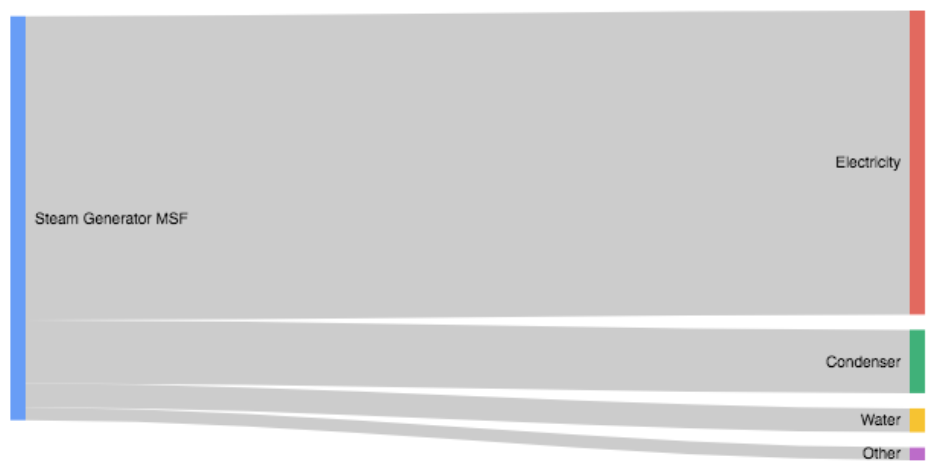
\includegraphics[width=\textwidth]{SankeySG3.PNG}
\caption{\small \sl The Mass exergy allocation in the configuration with the \ac{msf} system after the steam generator made using Google Charts}
\label{SankeySG}
\centering
\end{figure*}

\begin{figure*}[h!]
\centering
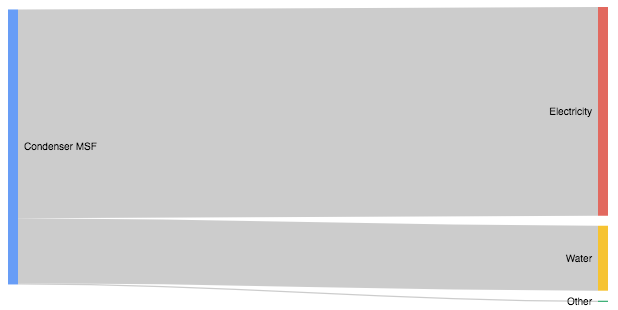
\includegraphics[width=\textwidth]{Condenser.png}
\caption{\small \sl The Mass exergy allocation in the configuration with the \ac{msf} system after the condenser made using Google Charts}
\label{SankeyC}
\centering
\end{figure*}
\begin{figure*}[h!]
\centering
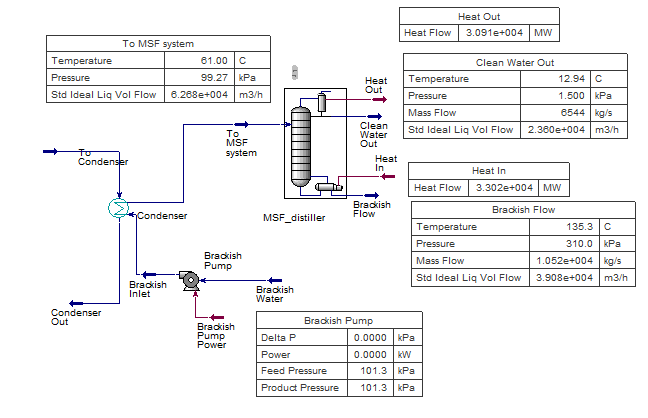
\includegraphics[width=\textwidth]{PowerCycle.png}
\caption{\small \sl The Mass exergy allocation in the configuration with the \ac{msf} system after the steam generator made using Google Charts}
\label{SankeyPC}
\centering
\end{figure*}
\clearpage

\subsubsection{Minimal Water Requirements}
Annually, Palo Verde uses approximately 75,700 acre feet of water per year.  To ensure that Palo Verde continues to have sufficient water for operations from groundwater resources, the models developed have calculated the resources required to meet 20\% of the annual water demand for the plant, approximately 15,140 acre feet per year, or 1.728 acre feet, $2131.45 \hspace{.17 cm} m^3$, per hour if kept running all year. While the water output will likely vary depending on the electric grid demand, the average output would need to be $2131.45 m^3$ for the system to produce 20\% of the water demand for Palo Verde. Meeting this minimum demand is feasible for both the reverse osmosis and the MSF systems.

 The first row of table \ref{MSF-X} is the configuration with extra heat sent to the condenser as can be seen in \ref{MSF_condense}.  The second and third rows of table \ref{MSF-X} reflect the values associate with the configuration presented in \ref{MSF_SG}. To achieve the minimal amount of water demand required splitting about 3.4\% of the water from the power cycle. Due to the requirement of sending at least 80\degree C water to the condenser, not as much electricity is generated when the heat is taken directly from the condenser. The third row in \ref{MSF-X} attempts to demonstrate a more equal comparison with the second configuration producing approximately the same amount of water. Both systems have approximately the same overall exergy destruction equivalent to general power cycle exergy losses, no matter if there is a thermally coupled water purification system or just the turbines generating electricity.   The SW-L reverse osmosis systems require significantly less electricity than the thermally coupled systems required in the form of heat.  While the RO systems generated significantly less water than the MSF system coupled to the condenser, the SW-L RO system overall had a greater \$/exergy value as can be seen in table \ref{RO-X}.

\begin{table}[h!]
\centering
\caption{Exergy analysis of the MSF system}
\begin{tabular}{|l|l|l|l|l|l|l|}
\hline
\textbf{Description} &\multicolumn{1}{|c|}{\textbf{\begin{tabular}[c]{@{}c@{}}Input\\ Water\\ Temp\\ (C)\end{tabular}}} & \multicolumn{1}{c|}{\textbf{\begin{tabular}[c]{@{}c@{}}Distillation\\ Temp\\ (Celsius)\end{tabular}}} & \textbf{\begin{tabular}[c]{@{}l@{}}Power\\ Cycle\\ Efficiency\end{tabular}} & \textbf{\begin{tabular}[c]{@{}l@{}}Water\\ Generated\\ $\frac{m^3}{hr}$\end{tabular}} &  \textbf{\begin{tabular}[c]{@{}l@{}}Hourly\\ Total\\ Revenue\\ (\$/hr)\end{tabular}} & \textbf{\$/exergy} \\ \hline
 MSF from Condenser & 80.64 & 80  & 27.84\% &  29940 &	97434.18 &	92.21 \\ \hline
\begin{tabular}[c]{@{}l@{}}MSF 3.4\%\\ Split from\\ Power Cycle\end{tabular}& 289.4 & 80 & 27.67\% & 2139 & 88544.60 & 84.93\\ \hline
\begin{tabular}[c]{@{}l@{}}MSF 42\%\\ Split from\\ Power Cycle\end{tabular}& 289.4 & 80 & 16.31\% & 31360 & 58932.8 & 56.07\\\hline
\end{tabular}
\label{MSF-X}
\end{table}


\begin{table}[h!]
\centering
\caption{Reverse Osmosis Exergy Analysis values}
\begin{tabular}{|l|l|l|l|l|l|}
\hline
\multicolumn{1}{|c|}{\textbf{\begin{tabular}[c]{@{}c@{}}Type of\\ Pump\end{tabular}}} & \multicolumn{1}{c|}{\textbf{\begin{tabular}[c]{@{}c@{}}Number of\\ Pumps\end{tabular}}} & \textbf{\begin{tabular}[c]{@{}l@{}}Water\\ Generated\\ $\frac{m^3}{hr}$\end{tabular}} & \textbf{\begin{tabular}[c]{@{}l@{}}Hourly\\ Total\\ Revenue\\ (\$/hr)\end{tabular}} & \textbf{\$/exergy} \\ \hline
SW-S  & 52 & 2168.92  & 82123.94   & 78.97 \\ \hline
SW-L  & 11  & 2292.4     & 104486.30 & 100.47  \\ \hline
\end{tabular}
\label{RO-X}
\end{table}

To do a more even comparison, similar to what is performed in row 3 of table \ref{MSF-X}, table \ref{RO-H2O} displays the RO exergy analysis assuming approximately the same amount of water generated as the row one of \ref{MSF-X}. In this case, the SW-L pump has the best overall exergy economy of the reverse osmosis examples. Generating more or less water does not have a large impact on the overall exergy economy comparisons.  Similar to the load following analysis, the reverse osmosis examples do slightly better than the MSF configurations.The RO systems are more controllable in allocating electricity. The exergy value for the RO systems is greater due to the high price placed on electricity as opposed to water.  The RO systems are able to produce the necessary amount of water for little electricity while selling the remaining electricity to the grid.

\begin{table}[h!]
\centering
\caption{Reverse Osmosis Exergy Analysis Values Generating similar amounts of water as generated in the MSF system}
\begin{tabular}{|l|l|l|l|l|l|}
\hline
\multicolumn{1}{|c|}{\textbf{\begin{tabular}[c]{@{}c@{}}Type of\\ Pump\end{tabular}}} & \multicolumn{1}{c|}{\textbf{\begin{tabular}[c]{@{}c@{}}Number of\\ Pumps\end{tabular}}} & \textbf{\begin{tabular}[c]{@{}l@{}}Water\\ Generated\\ $\frac{m^3}{hr}$\end{tabular}} &  \textbf{\begin{tabular}[c]{@{}l@{}}Hourly\\ Total\\ Revenue\\ (\$/hr)\end{tabular}} & \textbf{\$/exergy} \\ \hline
SW-S  & 715   & 29820 & 100380  &  96.52 \\ \hline
SW-L & 144   & 30010  & 100700  & 96.82  \\ \hline
\end{tabular}
\label{RO-H20}
\end{table}

	Given the average prices assumed in this model, the greatest amount of revenue between the two purification systems clearly comes from the reverse osmosis system.  The model assumes a much higher value for the electricity than for the water generated.  If trends continue, with renewables at times pushing down the price of electricity to negative values zero, generating water will result in greater revenue at times.  The model also assumes the 2018 purchase price of water for Palo Verde Generating Station. The predicted price of water is assumed to double by 2025 \cite{Brown2018}.  In that event, Palo Verde could sell water to the public at significantly higher prices, resulting in water production profit competing with electricity production profit at times.  As mentioned previously, the cost of water to Tucson residents averaged around \$1.42 per cubic meter, over thirteen times more than the price assumed for this study \cite{CityofTucson2017}. At the moment, assuming average values for water costs and wholesale electricity price, the RO system both brings in significantly greater revenue and is much simpler to couple and operate.


\section{Exergy Analysis Conclusions}

The exergy analysis approach taken in this research is not the traditional approach used to evaluate costs for the exergy losses at each of the components in the system.  This research focuses on the revenues from the various sources, as what is driving the purpose for the coupling in the first place.  The primary reason \ac{aps} is evaluating water purification systems in large part is not to minimize costs, but to maximize the possible revenue.  APS plans to use the water production facility to balance output when the price of electricity decreases to a point where water production makes more sense, which is dependent on the price of water and the price of electricity, not the cost of generation. The losses from the power cycle were very similar in each of the cases evaluated here, making a more traditional exergy analysis less relevant. The electrically coupled reverse osmosis system makes the best overall sense when strictly evaluating the revenue.  The reverse osmosis system is able to produce sufficient amounts of water to meet Palo Verde's water needs, is easier to operate, and makes the greatest overall revenue.

\begin{table}[h!]
\centering
\caption{Overall conclusions from the analysis on the \$/exergy of the various water purification configurations}
\label{}
\begin{tabular}{|l|l|l|l|}
\hline
\textbf{Characteristic}                                                               & \multicolumn{1}{c|}{\textbf{MSF-SG}}                                                                & \multicolumn{1}{c|}{\textbf{\begin{tabular}[c]{@{}c@{}}MSF\\ Condenser\end{tabular}}}              & \multicolumn{1}{c|}{\textbf{RO}}                                                                 \\ \hline
\textbf{Complexity}                                                                   & \begin{tabular}[c]{@{}l@{}}Greatest\\ Configuration\\ Change\end{tabular}                           & \begin{tabular}[c]{@{}l@{}}Potentially less\\ Configuration\\ Change\end{tabular}                  & Least Complex                                                                                    \\ \hline
\textbf{Flexibility}                                                                  & \begin{tabular}[c]{@{}l@{}}Able to take a\\ wide range \\of loads\end{tabular}                          & \begin{tabular}[c]{@{}l@{}}Requires $\sim$10\%\\ load reduction\\ as minimum\end{tabular}                       & \begin{tabular}[c]{@{}l@{}}Flexible to the\\ point of the\\ capacity of the\\ plant\end{tabular} \\ \hline
\textbf{Ideal usage}                                                                  & \begin{tabular}[c]{@{}l@{}}System that\\ has a wide variance\\ in production\\ demand\end{tabular} & \begin{tabular}[c]{@{}l@{}}System that \\ emphasizes a\\ large volume of water \\ production\\with at least 10\% \\ energy allocation\end{tabular} & \begin{tabular}[c]{@{}l@{}}Best Overall \\ \& Systems\\ that require\\ minimal \\ complexity\end{tabular}  \\ \hline
\end{tabular}
\end{table}


\clearpage



\section{Dynamic Analysis using \ac{raven}}


The literature review presented in this thesis emphasized the importance of dynamic modeling in analyzing a \ac{nrhes}. Currently, about 10\% of the electricity consumed by retail customers in the \ac{aps} service area comes from renewable energy, primarily solar \cite{ArizonaPublicService2018}.  By 2025, 15\% of all of APS's electricity generation is mandated to come from renewables \cite{UtilitiesDivision}. As can be seen in figure \ref{solargen}, the trend is for greater variable solar generation implementation and overall generation. One of the primary benefits of coupling a water purification system to the Palo Verde power plant is to flexibly operate the plant when there is little grid demand. By analyzing what kinds of daily fluctuations are likely, this study includes a brief analysis of one of the major benefits of coupling the system. In order to perform a quasi dynamic analysis, \ac{raven} is used to determine the one or two major times in the day when energy demand shifts significantly. To determine what demand looks like for a standard day in each season, \ac{raven} is first used to analyze electricity demand data, then to generate typical demand curves for each of the seasons. The \ac{aps} demand data come from the \ac{eia} and includes total hourly demand data from July 2015 through May 2018. The generated data is used as the basis for establishing the total electric demand for a standard day in each season in the APS territory.  The dates for the beginning and end of each season were pulled from the Farmers' Almanac \cite{Almanac}.

While there is not hourly generation data available for the solar added to the grid, there is total monthly generation data. As can be seen in figure \ref{solargen}, in 2017 in Arizona, the total amount of solar generated went from a low in January of 313.55 thousand MWh to 756.46 thousand MWh \cite{Eia2018}.  Due to Arizona taking some of California's overproduction it is also important to note the amount of solar generated in the neighboring state.  California went from a low of 1495.85 thousand MWh in January 2017 to 3888.38 thousand MWh in June 2017\cite{Eia2018}. The change between different times of the year is substantial. For Arizona and California, the increased generation from solar does match the increased demand from air conditioning use, which would ease the challenges of having a variable load.  In places that do not need air conditioning, there would likely be a greater mismatch between the solar generation and the demand.

\begin{figure*}[t!]
    \centering
    \begin{subfigure}[b]{\textwidth}
        \centering
        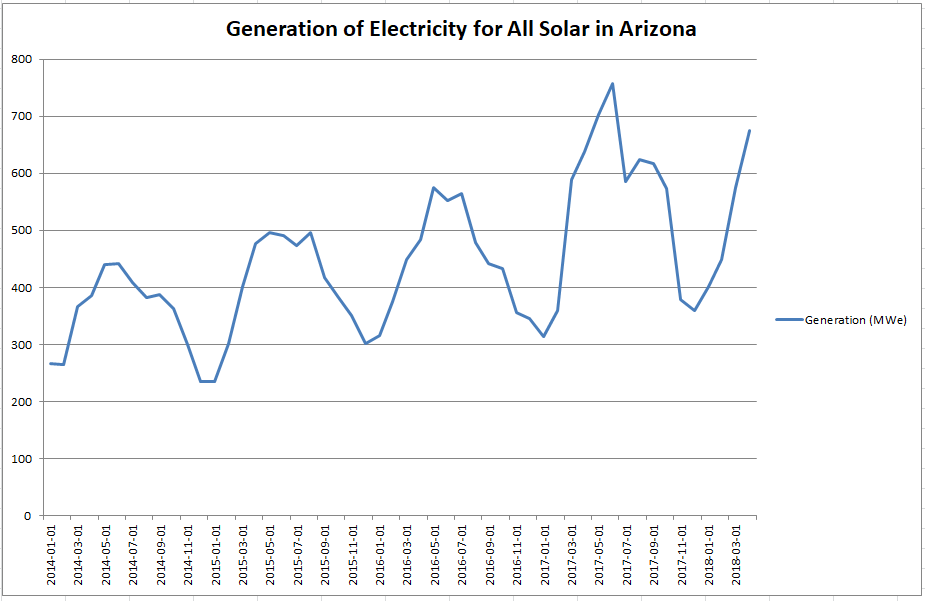
\includegraphics[height=1.8in]{AZ_solar_gen.PNG}
        \caption{\small \sl Arizona solar generation is increasing rapidly each year.  There is greater difference between the summer and winter generation.}
    \end{subfigure}
     \hfill
    \begin{subfigure}[t]{\textwidth}
        \centering
        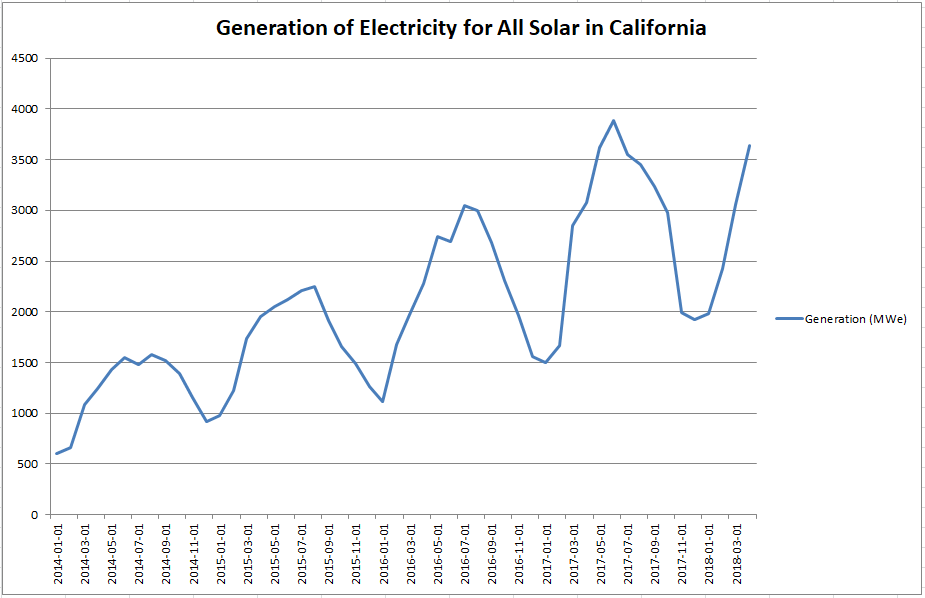
\includegraphics[height=1.8in]{Calif_generation.PNG}
        \caption{\small \sl California solar generation is increasing rapidly each year.  There is greater difference between the summer and winter generation.}
    \end{subfigure}
    \hfill
    \caption{\small \sl Monthly solar generation data for Arizona and California. Data from January 2014 until April 2018 sourced from the EIA \cite{EIA2017}}
    \label{solargen}
\end{figure*}

\subsection{Demand Generation Approach}
RAVEN was introduced in the discussion surrounding the current \ac{nrhes} modeling approaches.  As described previously, RAVEN was initially built for probabilistic risk assessment.  It has been used to generate synthetic data for wind demand in prior \ac{nrhes} modeling as well as sensitivity analyses and uncertainty analyses.  For this analysis, RAVEN is used to generate synthetic data corresponding to the demand for APS in various seasons.  Due to the changes in weather and hours of sunlight, consumption of electricity can vary greatly between the seasons. For example, as can be seen in figure \ref{SyntheticAverage}, the overall demand for Arizona is greatest in the summer, likely due to air conditioning use. RAVEN uses real historic data to train one of the selection of \ac{roms}, then generates new data with similar statistical qualities, such as the mean and the standard deviation. In this research, the \ac{arma} ROM is trained  to generate the data based on the\ac{eia} demand data and then produced synthetic data.


ARMA is comprised of two parts: an autoregressive and a moving average part.  The autoregressive part uses previous data for the time of day and demand to predict future values for the demand at that time of day. The moving average part includes the error term in the data as a linear combination of current and previous error terms. As can be seen in the raw data graphs in figure \ref{RawDemand}, each season has many different demand paths. The ARMA model applied in this research uses a Monte Carlo Sampler. A Monte Carlo approach generates inputs. In this case, the inputs could be the demand for a given time and the computations could surround the errors associated with that input from the average. The ARMA model then generates 10 different possible demand curves for each of the seasons.  The generated demand curves have very similar means and standard deviation values as those found in the raw data. The ARMA model generates synthetic data which shows general trends found in the demand for each of the seasons.

The graphs in figure \ref{RawDemand} show the various daily demand curves for each season. The raw data curves display the actual input data from the \ac{eia}. Further investigation is necessary to validate the data taken from the EIA data base. There can be anomalous days in the real data, therefore generating the synthetic data can provide a more generally applicable demand data for any given day in the season.  Each of the graphs in figure \ref{SyntheticAverage} display ten synthetically generated curves. As shown in \ref{RawDemand}(a), total demand is high in the middle of the day, when the sun is likely to be hottest and therefore electricity demand greatest. Winter has a different overall shape possibly due to not having as a much of a demand for air conditioning.  A typical change in demand can be determined using the synthetically generated curves. From the synthetically generated curves, the largest demand change can be approximated to include in the analysis of the coupled water purification systems.

Figures \ref{RawDemand} and \ref{SyntheticAverage} show the total demand, not the net demand, where the renewable generation would be subtracted from the total.  Future work should include the net demand data to show how renewables are impacting the daily demand curves in each season.

\begin{figure*}[t!]
    \centering
    \begin{subfigure}[b]{\textwidth}
        \centering
        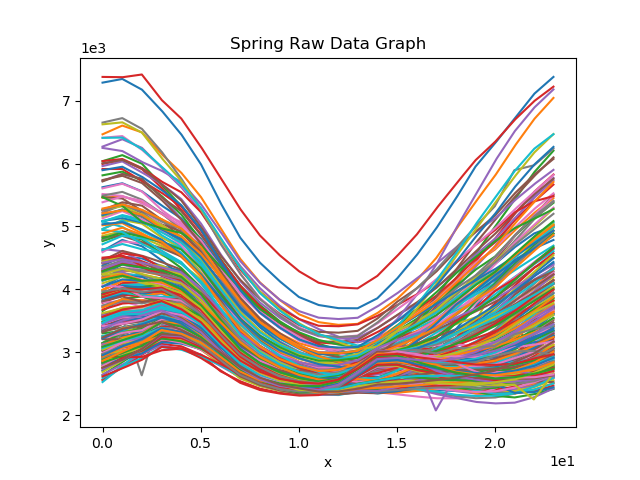
\includegraphics[height=1.8in]{Spring_Raw_Data_Graph_line.png}
        \caption{\small \sl Raw \ac{aps} Spring Demand Data. x is in hours (the 24 hours in a day). y is APS's electric demand in MWe.}
    \end{subfigure}
     \hfill
    \begin{subfigure}[t]{\textwidth}
        \centering
        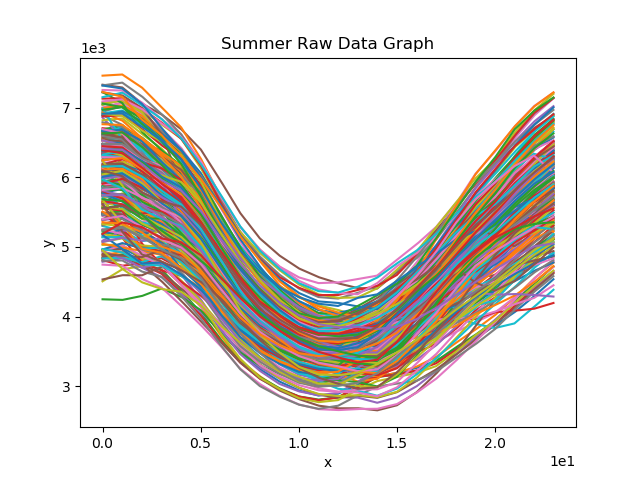
\includegraphics[height=1.8in]{Summer_Raw_Data_Graph_line.png}
        \caption{\small \sl Raw \ac{aps} Summer Demand Data. x is in hours. y is APS's electric demand in MWe.}
    \end{subfigure}
    \vskip\baselineskip
    \begin{subfigure}[t]{\textwidth}
        \centering
        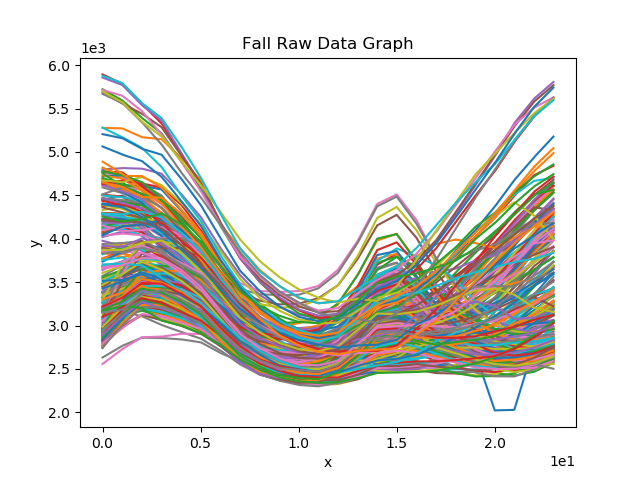
\includegraphics[height=1.8in]{Fall_Raw_Data_Graph_line.png}
        \caption{\small \sl Raw \ac{aps} Fall Demand Data. x is in hours. y is APS's electric demand in MWe.}
    \end{subfigure}
    \quad
    \begin{subfigure}[t]{0.9\textwidth}
        \centering
        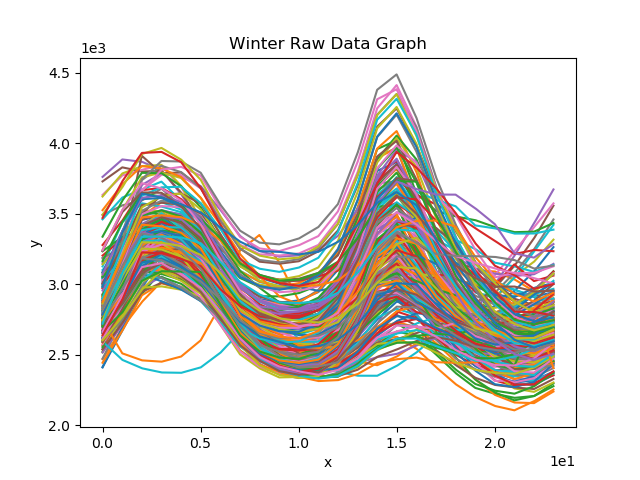
\includegraphics[height=1.8in]{Winter_Raw_Data_Graph_line.png}
        \caption{\small \sl Raw \ac{aps} Winter Demand Data. x is in hours. y is APS's electric demand in MWe.}
    \end{subfigure}

    \caption{\small \sl Raw data showing general Arizona Public Service Demand from the EIA from July 1st, 2015 to May 18, 2018}
    \label{RawDemand}
\end{figure*}

\begin{figure*}[t!]
    \centering

    \begin{subfigure}[b]{0.9\textwidth}
        \centering
        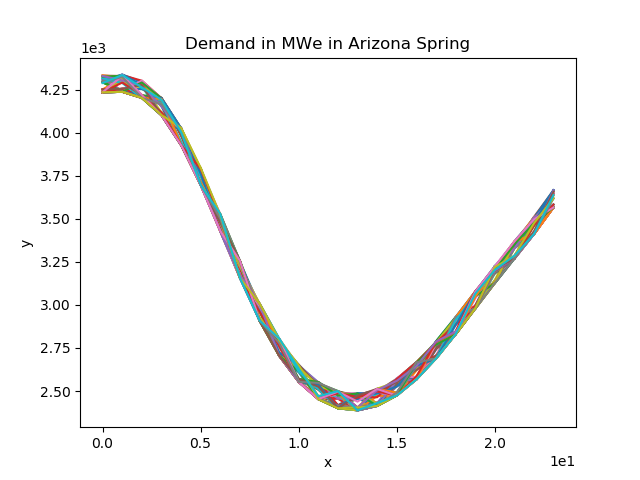
\includegraphics[height=1.8in]{Demand_in_MWe_in_Arizona_Spring_line.png}
        \caption{\small \sl Spring \ac{aps} Demand Data. x is in hours (the 24 hours in a day). y is APS's electric demand in MWe.}
    \end{subfigure}
     \hfill
    \begin{subfigure}[t]{0.9\textwidth}
        \centering
        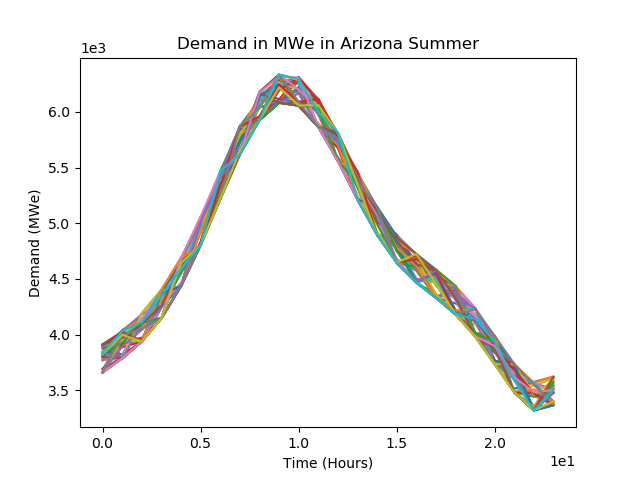
\includegraphics[height=1.8in]{Demand_in_MWe_in_Arizona_Summer_line.png}
        \caption{Synthetic \ac{aps} Summer Demand Data. x is in hours. y is APS's electric demand in MWe.}
    \end{subfigure}
    \vskip\baselineskip
    \begin{subfigure}[t]{0.9\textwidth}
        \centering
        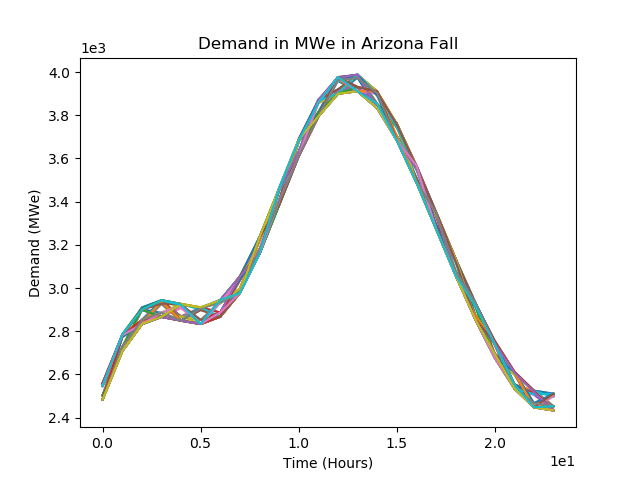
\includegraphics[height=1.8in]{Demand_in_MWe_in_Arizona_Fall_line.png}
        \caption{\small \sl Synthetic \ac{aps} Fall Demand Data. x is in hours. y is APS's electric demand in MWe.}
    \end{subfigure}
    \quad
    \begin{subfigure}[t]{0.9\textwidth}
        \centering
        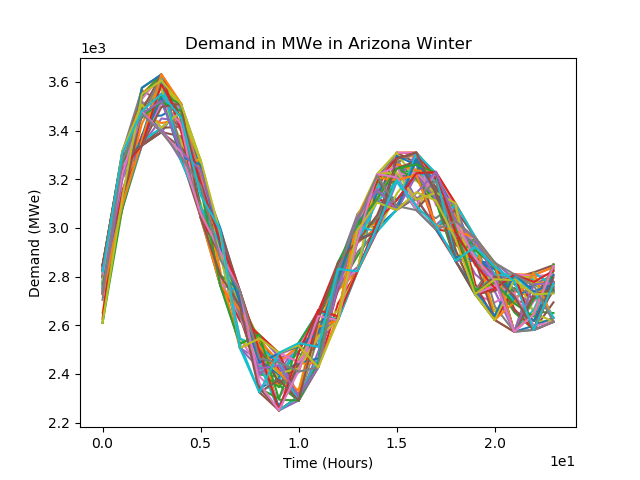
\includegraphics[height=1.8in]{Demand_in_MWe_in_Arizona_Winter_line.png}
        \caption{\small \sl Synthetic \ac{aps} Winter Demand Data. x is in hours. y is APS's electric demand in MWe.}
    \end{subfigure}
    \caption{\small \sl Cleaned up Synthetic Data showing general Arizona Public Service Demand}
    \label{SyntheticAverage}
\end{figure*}

\clearpage

\begin{table}[h!]
\centering
\caption{Approximate average values for demand change in Arizona for each season}

\begin{tabular}{|l|l|l|l|l|l|}
\hline
\multicolumn{1}{|c|}{\textbf{Season}} & \multicolumn{1}{c|}{\textbf{\begin{tabular}[c]{@{}l@{}}Peak\\ Demand\\ (MWe)\end{tabular}}} & \textbf{\begin{tabular}[c]{@{}l@{}}Minimum\\ Demand\\ (MWe)\end{tabular}} & \textbf{\begin{tabular}[c]{@{}l@{}}Change in\\ Demand\\ (MWe)\end{tabular}} & \textbf{\begin{tabular}[c]{@{}l@{}}Local\\ Minimums\\ (MWe)\end{tabular}} & \textbf{\begin{tabular}[c]{@{}l@{}}Change in \\ Local\\Demand (MWe)\end{tabular}} \\ \hline
Spring                                & 4300                                      & 2320                                                              & 1980                                                                & N/A                                                               & N/A                                                                        \\ \hline
Summer                                & 6400                                      & 3500                                                              & 2900                                                                & N/A                                                               & N/A                                                                        \\ \hline
Fall                            & 3900                                      & 2350                                                              & 1550                                                                & 2950                                                              & 950                                                                        \\ \hline
Winter                                & 3500                                      & 2450                                                              & 1050                                                                & 2500                                                              & 1000                                                                       \\ \hline
\end{tabular}
\label{DemandChange}
\end{table}


\subsection{Fluctuation Analysis}
As figures \ref{SyntheticAverage}, \ref{RawDemand}, and table \ref{DemandChange} demonstrate, the load change over a day would generally require that all of the electricity be diverted from the APS-owned load from Palo Verde if following strictly with the nuclear generation.  Since the demand curves typically decrease and increase over several hours, the load would have to be shifted to water production in portions over the day if load following just with Palo Verde.  The various exergy and revenue outcomes from the thermally and electrically coupled systems at different rates of load following have already been detailed in tables \ref{LoadFollow}, \ref{SW-S} and \ref{SW-L}. The tendency for the demand to shift gradually would suggest a benefit to electrically coupling, which does not have thermal hydraulic feedbacks from shifting. Overall, if load following just with the load APS owns from Palo Verde, there would not be sufficient change, even if decreasing the load to zero to load follow in any season besides from winter.

APS owns and operates natural gas and coal power plants which are the more traditional generation sources that vary output. Looking at figure \ref{SyntheticAverage}(d) reflecting the total winter demand hovering below 2000 MWe on some days, it is very plausible that sometimes renewable generation will make up over 900 MWe during that period and APS will have too much generation even with all the coal and natural gas removed from the grid.

\section{Conclusions}
\begin{itemize}
\item The SW-L 630 RO system had the greatest overall revenue and \$/exergy values.
\item The reverse osmosis systems all had greater values for \$/exergy than the MSF configurations.
\item The electricity and water costs which result in greater overall revenue with the reverse osmosis configurations are well within the realistic price range for the two commodities.
\item Palo Verde Generating Station will need to flexibly operate to deal with the increasing level of variable penetration in both Arizona and California.
\item Generating sufficient water to meet 20\% of Palo Verde's water needs does not require a lot of load following.
\item The water purification systems that are reasonably sized would not require as much power as Palo Verde needs in order to make up for the overproduction on the grid at times.
\item The overall question of what the thermodynamic and economic benefits of thermally coupling a system requires using the exact same technology as the industrial process. The analysis done here ends up comparing two separate industrial processes and thus does not evaluate the benefits of a thermally versus an electrically coupled system.
\end{itemize}
